% ============================================================
%  Global Undergraduate Awards 2026 - Engineering Category
%  Single-file submission. Place in a folder with:
%    - figures/   (all images referenced below)
%    - references/references.bib
%  Compile: pdflatex -> bibtex -> pdflatex -> pdflatex
%  ANONYMISED: no names, institution, supervisor, or IDs.
% ============================================================
\documentclass[11pt,a4paper]{article}
\usepackage[margin=1in]{geometry}
\usepackage{lmodern}
\usepackage[protrusion=true,expansion=true]{microtype}
\usepackage{titling}
\usepackage{enumitem}
\usepackage{longtable}
\usepackage{booktabs}
\usepackage{graphicx}
\usepackage{tabularx}
\usepackage{caption}
\usepackage{tocloft}
\usepackage{float}
\usepackage{amsmath}
\usepackage{amssymb}
\usepackage{xcolor}
\usepackage{hyperref}
\usepackage{fancyhdr}
\usepackage{pgfplots}
\pgfplotsset{compat=1.18}
\usepackage{subcaption}
% Look for figures in a figures/ subfolder OR flat in the same folder.
\graphicspath{{figures/}{./}}

\setlength{\cftbeforesecskip}{8pt}
\setlength{\cftbeforesubsecskip}{4pt}

% Anonymised hyperref metadata (no author).
\hypersetup{
    colorlinks=true,
    linkcolor=black,
    citecolor=black,
    urlcolor=black,
    pdfborder={0 0 0},
    pdftitle={TAMRA - Embodied AI and Hybrid Hardware Synthesis for a Low-Cost Autonomous Service Robot},
    pdfauthor={},
    pdfsubject={},
    pdfkeywords={}
}

% Headers/footers (neutral running title; no institution).
\pagestyle{fancy}
\fancyhf{}
\fancyhead[L]{\small\textit{\leftmark}}
\fancyhead[R]{\small\textit{TAMRA: Autonomous Service Robot}}
\fancyfoot[C]{\thepage}
\renewcommand{\headrulewidth}{0.4pt}
\renewcommand{\footrulewidth}{0pt}
\renewcommand{\sectionmark}[1]{\markboth{#1}{}}
\fancypagestyle{plain}{
    \fancyhf{}
    \fancyfoot[C]{\thepage}
    \renewcommand{\headrulewidth}{0pt}
}

\begin{document}

% ============================================================
% TITLE PAGE  (anonymised)
% ============================================================
\begin{titlepage}
\centering
\vspace*{3cm}

{\Huge\textbf{T.A.M.R.A.}}\\[0.5cm]
{\LARGE\textbf{Embodied AI and Hybrid Hardware Synthesis for a\\[0.2cm] Low-Cost Autonomous Service Robot}}\\[1.0cm]
{\large Task-Agnostic Modular Robotic Apparatus}

\vspace{2.5cm}

{\large Final Year Project --- Bachelor of Engineering}\\[0.3cm]
{\normalsize Electrical \& Computer Engineering}

\vspace{1.5cm}

{\normalsize Academic Year 2025--2026}

\vfill

{\small Word count (body, excluding abstract, references, tables and captions): \textbf{$\approx$8{,}200} words.}\\
{\small This entry has been anonymised for the Global Undergraduate Awards.}

\end{titlepage}

% ============================================================
% ABSTRACT
% ============================================================
\newpage
\thispagestyle{empty}
\section*{Abstract}
\addcontentsline{toc}{section}{Abstract}

A service robot becomes genuinely useful only when it can navigate autonomously, converse naturally, and plan multi-step tasks --- yet commercial platforms deliver these capabilities in isolation and at institutional cost, and their integration onto a single affordable system remains largely unexplored. This work presents an integrated framework unifying LiDAR-based autonomous navigation, large-language-model semantic task orchestration, and real-time conversational interaction on one low-cost mobile platform, and validates it empirically. The central contribution is a semantic task orchestrator that translates free-form spoken commands into typed, multi-step mission plans --- navigate, speak, display, photograph --- streamed to an on-board mission engine that begins executing the first action before the full plan is generated, minimising perceived latency. Component selection across five subsystems was governed by the Analytic Hierarchy Process (consistency ratio 0.04), and localisation fuses LiDAR, inertial, and odometric data through an extended Kalman filter. The realised system was characterised through controlled integration tests: end-to-end voice-to-motion latency of $1.55 \pm 0.31$\,s ($n=20$), telemetry round-trip of $159 \pm 30$\,ms ($n=30$), and reliable generation of executable multi-waypoint missions across fifteen commands of increasing complexity. The complete platform --- including a locally fabricated ergonomic body shell developed through a structured design pipeline --- was realised for approximately USD~3{,}200, a 73\% reduction against the nearest comparable commercial system, which offers no equivalent combination of capabilities. These results demonstrate that research-grade embodied-AI integration is achievable without proprietary platforms or institutional-scale budgets, lowering the barrier to autonomous service robotics in resource-constrained settings such as healthcare.

\vspace{0.4cm}
\noindent\textbf{Keywords:} Autonomous Mobile Robots; Embodied AI; LLM Task Orchestration; LiDAR SLAM; ROS~2; Human--Robot Interaction; Sensor Fusion; Healthcare Robotics.

% ============================================================
% DECLARATION OF AI USE  (honest, anonymised)
% ============================================================
\newpage
\thispagestyle{empty}
\section*{Declaration on the Use of Generative AI}
\addcontentsline{toc}{section}{Declaration on the Use of Generative AI}

\noindent Generative AI tools were used during the preparation of this report to assist with literature-synthesis, prose refinement, and code documentation. The authors reviewed and edited all such output and take full responsibility for the accuracy, integrity, and originality of the work. Separately, where AI methods form part of the engineering work itself --- specifically a generative concept-rendering and image-to-3D mesh step in the body-shell design pipeline, and the large language model used as the orchestration component --- these are described, measured, and critically evaluated within the body of the report rather than relied upon uncritically; in particular, the AI-generated mesh required substantial parametric reconstruction before it was fabrication-ready (Section~\ref{sec:implementation}).

% ============================================================
% ACRONYMS
% ============================================================
\newpage
\thispagestyle{empty}
\section*{Acronyms}
\addcontentsline{toc}{section}{Acronyms}

\begin{tabular}{@{}ll@{}}
\toprule
\textbf{Acronym} & \textbf{Description} \\
\midrule
AHP & Analytic Hierarchy Process \\
AMR & Autonomous Mobile Robot \\
API & Application Programming Interface \\
ASR & Automatic Speech Recognition \\
EKF & Extended Kalman Filter \\
HRI & Human--Robot Interaction \\
IMU & Inertial Measurement Unit \\
LiDAR & Light Detection and Ranging \\
LLM & Large Language Model \\
MQTT & Message Queuing Telemetry Transport \\
ROS & Robot Operating System \\
SLAM & Simultaneous Localization and Mapping \\
SSE & Server-Sent Events \\
TTS & Text-to-Speech \\
\bottomrule
\end{tabular}

% ============================================================
% TABLE OF CONTENTS / LISTS
% ============================================================
\newpage
\tableofcontents
\newpage
\listoffigures
\listoftables
\newpage

\setcounter{page}{1}

% ============================================================
% 1. INTRODUCTION
% ============================================================
\section{Introduction}
\label{sec:introduction}

Modern healthcare systems worldwide face an urgent mandate to deliver safe, accessible, and high-quality care to growing populations. The post-pandemic era has highlighted critical vulnerabilities: the risk of infection during routine contact, the strain on medical staff, and the logistical burden of managing hospital wards~\cite{frontiers2024}. A significant portion of nursing time is spent on non-clinical logistics; this manual workload reduces patient-care time and increases staff exposure to infectious environments. This project introduces an autonomous robotic platform designed to automate routine service tasks, validated in a healthcare context but architected to generalise across any service environment.

\subsection{Problem Statement}
Oman's healthcare system reaches the great majority of the population~\cite{alsheikhly2006}, yet geographic distance and resource constraints create barriers to timely care for underserved groups. Existing telepresence solutions often rely on manual control and lack the ability to engage users in even basic dialogue, increasing clinician workload and offering a less effective experience for patients in rural areas or with mobility limitations. There is a need for an affordable mobile platform that combines autonomous navigation, natural interaction, item delivery, and telepresence in one system.

\subsection{Motivation}
Patients frequently need attention that could be provided remotely if the right tools existed: children need reassurance when parents are absent, elderly patients need medication reminders and check-ins, and rural communities need specialist access without long journeys. The global demand for remote-care robotics is growing rapidly, and Oman's Vision~2040 explicitly calls for healthcare innovation that serves all citizens equally~\cite{alhinai2024}. Studies of telemedicine adoption in Oman show both promise and room for improvement~\cite{alsalmani2023,alshishtawy2013}. The aim of this project is to design and implement a smart, autonomous service robot with indoor navigation and on-device conversational interaction for ward corridors and bedside spaces.

\subsection{Objectives}
\begin{itemize}[leftmargin=*]
    \item Develop a robust autonomous navigation system capable of dynamic obstacle avoidance and SLAM in crowded indoor corridors.
    \item Engineer a secure telepresence interface enabling real-time, low-latency audio/visual consultations.
    \item Integrate an AI-driven interaction layer (using large language models) for natural-language task issuance, guidance, and reassurance.
    \item Validate the system in realistic scenarios, demonstrating autonomous delivery and remote-consultation cycles.
\end{itemize}

\subsection{Methodology}
The project began with a requirements analysis informed by a literature review and a needs assessment. Design alternatives for the hardware platform and software architecture were then evaluated and selected using the Analytic Hierarchy Process (AHP). Development followed an iterative prototyping cycle: establishing reliable teleoperation, implementing and refining autonomous navigation, and integrating conversational-AI orchestration. Finally, the integrated system was validated through unit, integration, and acceptance testing, measuring navigation accuracy, end-to-end latency, and orchestration reliability.

% ============================================================
% 2. BACKGROUND AND RELATED WORK  (condensed from lit. review)
% ============================================================
\section{Background and Related Work}
\label{sec:background}

\paragraph{Autonomous mobile robots in healthcare.}
Autonomous mobile robots (AMRs) are increasingly deployed for hospital logistics --- transporting medication, samples, linens, and meals --- to reduce repetitive staff workload and limit infection exposure~\cite{frontiers2024}. Beyond logistics, socially assistive robots have shown measurable value in patient engagement and elderly care, providing reminders, companionship, and a channel for remote presence~\cite{broekens2009}. The recurring barrier to adoption is cost: clinically capable platforms are expensive, and their interaction models are typically rigid.

\paragraph{Commercial service robots and the capability gap.}
Leading commercial service robots illustrate the gap this work targets. Delivery-and-guidance platforms such as PuduBot~2~\cite{pudubot2} and Keenon~M2~\cite{m2medical} excel at navigation and item transport but rely on scripted, menu-driven interaction; telepresence-capable medical units~\cite{peanutmedical} and cleaning robots~\cite{puducc1} are similarly locked to a single vertical with closed software. Across these platforms, conversational AI and flexible multi-step task planning are absent from the standard configuration, and prices range from roughly USD~12{,}000 to USD~47{,}500. None offers an open interface for adding research-grade conversational autonomy.

\paragraph{Navigation and localisation.}
For indoor service environments, LiDAR-based SLAM consistently outperforms purely visual approaches in cluttered, low-texture settings, achieving sub-10\,cm accuracy at modest computational cost~\cite{tourani2022}. Fusing LiDAR with inertial and wheel-odometry data through probabilistic state estimation further reduces drift over extended trajectories~\cite{doduc2024,thrun2005probabilistic}. The ROS~2 Nav2 stack provides a mature, well-supported framework for costmap-based planning and recovery behaviours in human-shared spaces~\cite{macenski2022ros2,macenski2023nav2}.

\paragraph{Conversational AI for human--robot interaction.}
Natural, low-friction interaction is decisive for acceptance of service robots by non-expert users~\cite{garingo2016}. The cost and latency of large-language-model (LLM) inference have fallen by orders of magnitude, making real-time, multimodal dialogue feasible without dedicated inference hardware~\cite{google2025pricing}, and domain-adapted medical models point toward future clinical decision support~\cite{medgemini2024}. The opportunity --- and the focus of this project --- is to use an LLM not merely as a chatbot but as a \emph{task orchestrator} that converts natural language into executable robot missions, bridging conversational AI and physical autonomy on an affordable platform.

% ============================================================
% 3. REQUIREMENTS SPECIFICATION  (condensed from ch.3)
% ============================================================
\section{Requirements Specification}
\label{sec:requirements}

Requirements are organised into customer requirements (high-level stakeholder needs), engineering requirements (quantifiable, testable specifications), and engineering constraints (operating boundaries). Each engineering requirement is mapped to one or more customer requirements for traceability.

\subsection{Customer Requirements}
\begin{itemize}[leftmargin=*]
    \item \textbf{CR1 --- Autonomous navigation and mobility.} Navigate corridors, rooms, and common areas without human intervention, avoiding static and dynamic obstacles.
    \item \textbf{CR2 --- Remote telepresence.} Enable high-quality remote video/audio for consultations, rounds, and family visits, providing a mobile presence for clinicians not at the bedside~\cite{garingo2016}.
    \item \textbf{CR3 --- Patient engagement.} Engage users through natural-language conversation for information, guidance, and reassurance, especially for paediatric and elderly populations.
    \item \textbf{CR4 --- Infection control and hygiene.} Use materials and surfaces compatible with standard hospital disinfection protocols~\cite{intel2024,sciencedirect2021}.
    \item \textbf{CR5 --- User-friendly interface.} Provide intuitive touchscreen, voice, and remote interfaces usable without technical training.
    \item \textbf{CR6 --- Continuous operation.} Operate through the working day with autonomous return-to-dock charging when battery is low.
\end{itemize}

\subsection{Engineering Requirements}
Engineering requirements translate the customer needs above into measurable, verifiable targets. Representative requirements for the navigation, interaction, and safety subsystems are given in Tables~\ref{tab:er_navigation}--\ref{tab:er_safety}; power-and-endurance and telepresence requirements (continuous operation of at least 4--6\,h, autonomous docking at 20\% battery with a 95\% success target, $\geq$720p/30\,fps video, and end-to-end audio latency below 200\,ms) are specified on the same basis.

\begin{table}[H]
\centering
\small
\begin{tabularx}{\linewidth}{|l|>{\raggedright\arraybackslash}X|l|>{\raggedright\arraybackslash}X|}
\hline
\textbf{ID} & \textbf{Specification} & \textbf{CR} & \textbf{Verification} \\
\hline
ER1.1 & Position accuracy of $\pm$20\,cm in mapped indoor environments & CR1 & Ground-truth positioning trials \\
\hline
ER1.2 & Maximum linear velocity of 0.5--1.0\,m/s in corridors (ISO~13482) & CR1 & Speed measurement tests \\
\hline
ER1.3 & Detect/avoid static and dynamic obstacles; detection range $\geq$3\,m, reaction $<$1\,s & CR1 & Obstacle-avoidance trials \\
\hline
ER1.4 & Minimum payload of 5\,kg for compute, sensors, and delivery items & CR2 & Load testing \\
\hline
\end{tabularx}
\caption{Navigation and mobility engineering requirements.}
\label{tab:er_navigation}
\end{table}

\begin{table}[H]
\centering
\small
\begin{tabularx}{\linewidth}{|l|>{\raggedright\arraybackslash}X|l|>{\raggedright\arraybackslash}X|}
\hline
\textbf{ID} & \textbf{Specification} & \textbf{CR} & \textbf{Verification} \\
\hline
ER3.1 & Interpret user intent in English and Arabic with $>$90\% accuracy on common queries & CR3 & Intent-classification testing \\
\hline
ER3.2 & Generate conversational responses within 3\,s of user input & CR3 & Response-latency measurement \\
\hline
ER3.3 & Speech recognition with word error rate $<$10\% in indoor noise & CR5 & ASR testing across speakers \\
\hline
\end{tabularx}
\caption{Social interaction and AI engineering requirements.}
\label{tab:er_ai}
\end{table}

\begin{table}[H]
\centering
\small
\begin{tabularx}{\linewidth}{|l|>{\raggedright\arraybackslash}X|l|>{\raggedright\arraybackslash}X|}
\hline
\textbf{ID} & \textbf{Specification} & \textbf{CR} & \textbf{Verification} \\
\hline
ER5.1 & Physical emergency-stop and software remote e-stop (ISO~13850) & CR1 & Functional e-stop testing \\
\hline
ER5.2 & Detect/avoid stairs, ramps $>$15$^\circ$, and drop-offs $>$2\,cm & CR1 & Edge-detection tests \\
\hline
ER5.3 & $>$95\% uptime during operational hours (excl. maintenance) & CR6 & Long-term reliability logging \\
\hline
\end{tabularx}
\caption{Safety and reliability engineering requirements.}
\label{tab:er_safety}
\end{table}

\subsection{Engineering Constraints}
The design was bounded by a tight academic budget; a single-academic-year timeline; operation on standard hospital Wi-Fi without dedicated infrastructure; compatibility with standard corridor widths ($\geq$1.5\,m) and indoor flooring; privacy-conscious handling of any captured data (aligned with HIPAA/GDPR principles, with no persistent storage of conversations or video); and reliance on commercially available, globally sourced components for long-term maintainability. These constraints steered the architecture toward mainstream, well-supported building blocks (ROS~2, common sensors, cloud AI APIs) rather than proprietary or region-specific hardware.

% ============================================================
% 4. SYSTEM CONCEPTUAL DESIGN  (condensed AHP from ch.4)
% ============================================================
\section{System Conceptual Design}
\label{sec:design}

\subsection{System Overview}
The robot is a mobile, autonomous platform for indoor service environments. Its functions are autonomous navigation, safe obstacle avoidance, point-to-point delivery, conversational interaction, and remote telepresence. The architecture follows a layered approach: a mobile base providing locomotion and payload capacity; a computing-and-control layer running ROS~2; a navigation-and-perception layer for localisation and obstacle detection; an intelligence layer built on a large language model; a communication-and-interface layer (tablet UI, web dashboard, voice); and a power-management layer with autonomous docking.

\subsection{Design Alternatives}
Three platform strategies were considered. \textbf{Alternative~A (commercial pre-built)} uses an off-the-shelf service robot: fast to deploy and reliable, but costly and difficult to customise mechanically. \textbf{Alternative~B (fully custom build)} fabricates the robot from individual components: maximally flexible and low in parts cost, but slow and high-risk within a fixed timeline. \textbf{Alternative~C (hybrid)} pairs a commercial mobile base providing proven navigation with custom-developed upper layers focused on AI-driven interaction and task management --- concentrating engineering effort on the project's differentiator while inheriting a safety-certified mobility base.

\subsection{Component Selection via AHP}
The Analytic Hierarchy Process (AHP) was used to make five independent design decisions systematically. For the platform decision, four criteria were weighted by pairwise comparison on Saaty's 1--9 scale (Table~\ref{tab:ahp_pairwise}), yielding the priority vector Cost~15\%, Development~Time~30\%, Customisability~8\%, Reliability~47\%, with a consistency ratio CR~$=0.04$ ($<0.10$, acceptable). Scoring each alternative against the criteria (Table~\ref{tab:ahp_scores}) produced the final platform scores in Table~\ref{tab:ahp_final}.

\begin{table}[H]
\centering
\caption{Platform criteria pairwise comparison matrix.}
\label{tab:ahp_pairwise}
\begin{tabular}{lcccc}
\toprule
\textbf{Criterion} & \textbf{Cost} & \textbf{Dev. Time} & \textbf{Custom.} & \textbf{Reliability} \\
\midrule
Cost & 1 & 1/3 & 3 & 1/5 \\
Development Time & 3 & 1 & 5 & 1/3 \\
Customisability & 1/3 & 1/5 & 1 & 1/7 \\
Reliability & 5 & 3 & 7 & 1 \\
\bottomrule
\end{tabular}
\end{table}

\begin{table}[H]
\centering
\caption{Platform alternative scores by criterion (1--9, higher is better).}
\label{tab:ahp_scores}
\begin{tabular}{lcccc}
\toprule
\textbf{Alternative} & \textbf{Cost} & \textbf{Dev. Time} & \textbf{Custom.} & \textbf{Reliability} \\
\midrule
A: Commercial   & 3 & 9 & 3 & 9 \\
B: Custom-Built & 9 & 3 & 9 & 5 \\
C: Hybrid       & 6 & 7 & 6 & 7 \\
\bottomrule
\end{tabular}
\end{table}

\begin{table}[H]
\centering
\caption{Final AHP scores for the robot platform.}
\label{tab:ahp_final}
\begin{tabular}{lc}
\toprule
\textbf{Alternative} & \textbf{Final Score} \\
\midrule
A: Commercial Pre-Built & 7.11 \\
B: Custom-Built Modular & 5.55 \\
\textbf{C: Hybrid Platform} & \textbf{6.76} \\
\bottomrule
\end{tabular}
\end{table}

\noindent Although Alternative~A scores marginally higher, the hybrid approach (C) was selected: the difference is small, and the hybrid strategy enables innovation in human--robot interaction --- the project's primary differentiator --- while inheriting proven navigation hardware.

A second AHP analysis selected the large language model. Four criteria (Performance~54\%, API~Familiarity~26\%, Latency~14\%, Cost~6\%; CR~$=0.05$) were applied to three candidates. Google Gemini~3~Flash scored highest (8.44) against GPT-5.2 (7.62) and GPT-4~Turbo (7.54), owing to its low latency for real-time interaction, multimodal input, and cost-effectiveness for extensive iteration. The remaining three decisions (computing platform, navigation approach, and localisation sensors) were resolved on the same basis; the consolidated outcome is given in Table~\ref{tab:ahp_summary}.

\begin{table}[H]
\centering
\caption{Final system component selection (AHP).}
\label{tab:ahp_summary}
\begin{tabular}{lll}
\toprule
\textbf{Component} & \textbf{Selected Option} & \textbf{Score} \\
\midrule
Robot Platform      & Hybrid (commercial base + custom AI) & 6.76 \\
Navigation Approach & LiDAR-based SLAM (Nav2)               & 7.95 \\
Localisation        & LiDAR + Odometry + IMU               & 8.20 \\
AI / LLM            & Google Gemini~3 Flash                & 8.44 \\
\bottomrule
\end{tabular}
\end{table}

\noindent These selections fixed the \emph{classes} of component rather than specific models. As Section~\ref{sec:implementation} details, procurement realities encountered at build time --- notably a supplier bankruptcy and the structural limits of educational bases --- forced a change of the specific mobile base while preserving the hybrid strategy and the criteria above.

\subsection{Functional Decomposition}
At the highest level the robot maps five input channels (voice, touch, remote dashboard, sensors, power) to five outputs (locomotion, voice response, display, telemetry, delivery), as shown in Figure~\ref{fig:level0-black-box}. The system decomposes into seven subsystems --- Mobility, Navigation, Perception, Intelligence, Task Management, Interface \& Communication, and Power Management --- whose interfaces and data flow are shown in Figure~\ref{fig:level1-subsystems}. The robot operates in a closed loop: perception feeds navigation and the intelligence layer; the intelligence layer interprets user intent into task requests; task management sequences these into navigation goals; mobility executes motion and returns odometry; and the interface and power subsystems expose status and manage charging.

\begin{figure}[H]
    \centering
    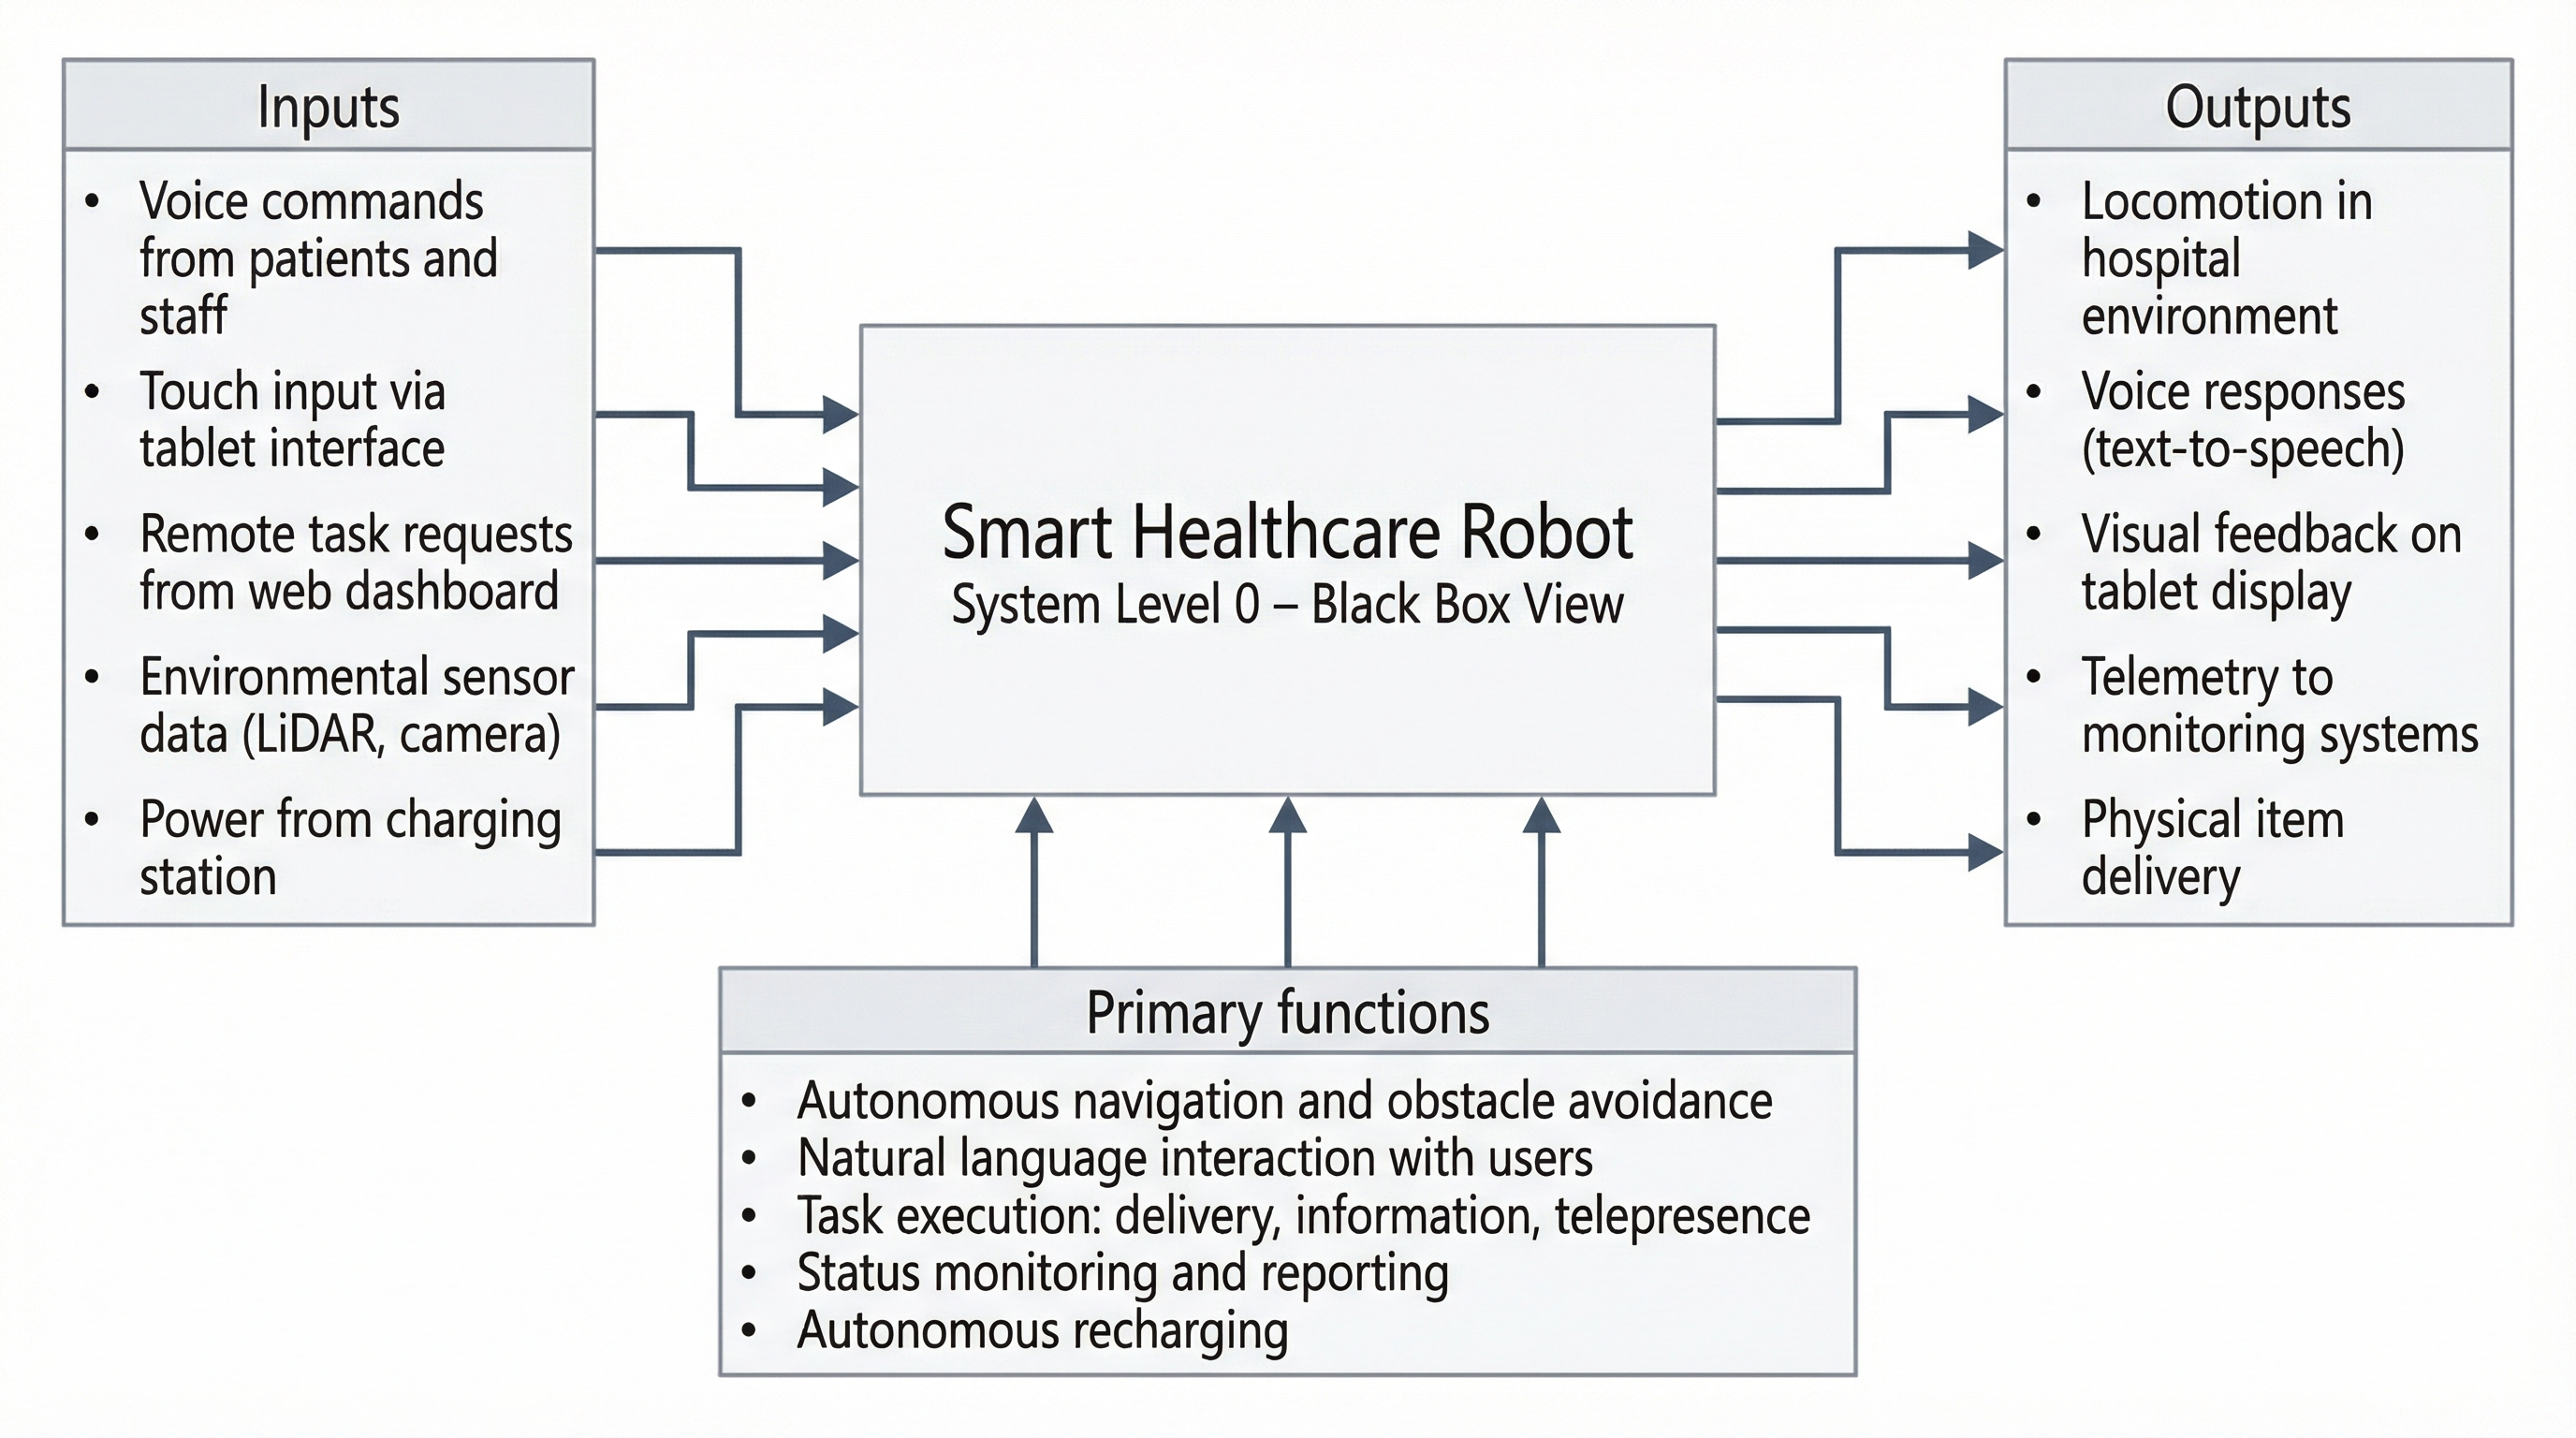
\includegraphics[width=0.95\textwidth]{level0-functional-view-1765609410658.png}
    \caption{System Level~0 black-box view: external inputs, outputs, and primary functions.}
    \label{fig:level0-black-box}
\end{figure}

\begin{figure}[H]
    \centering
    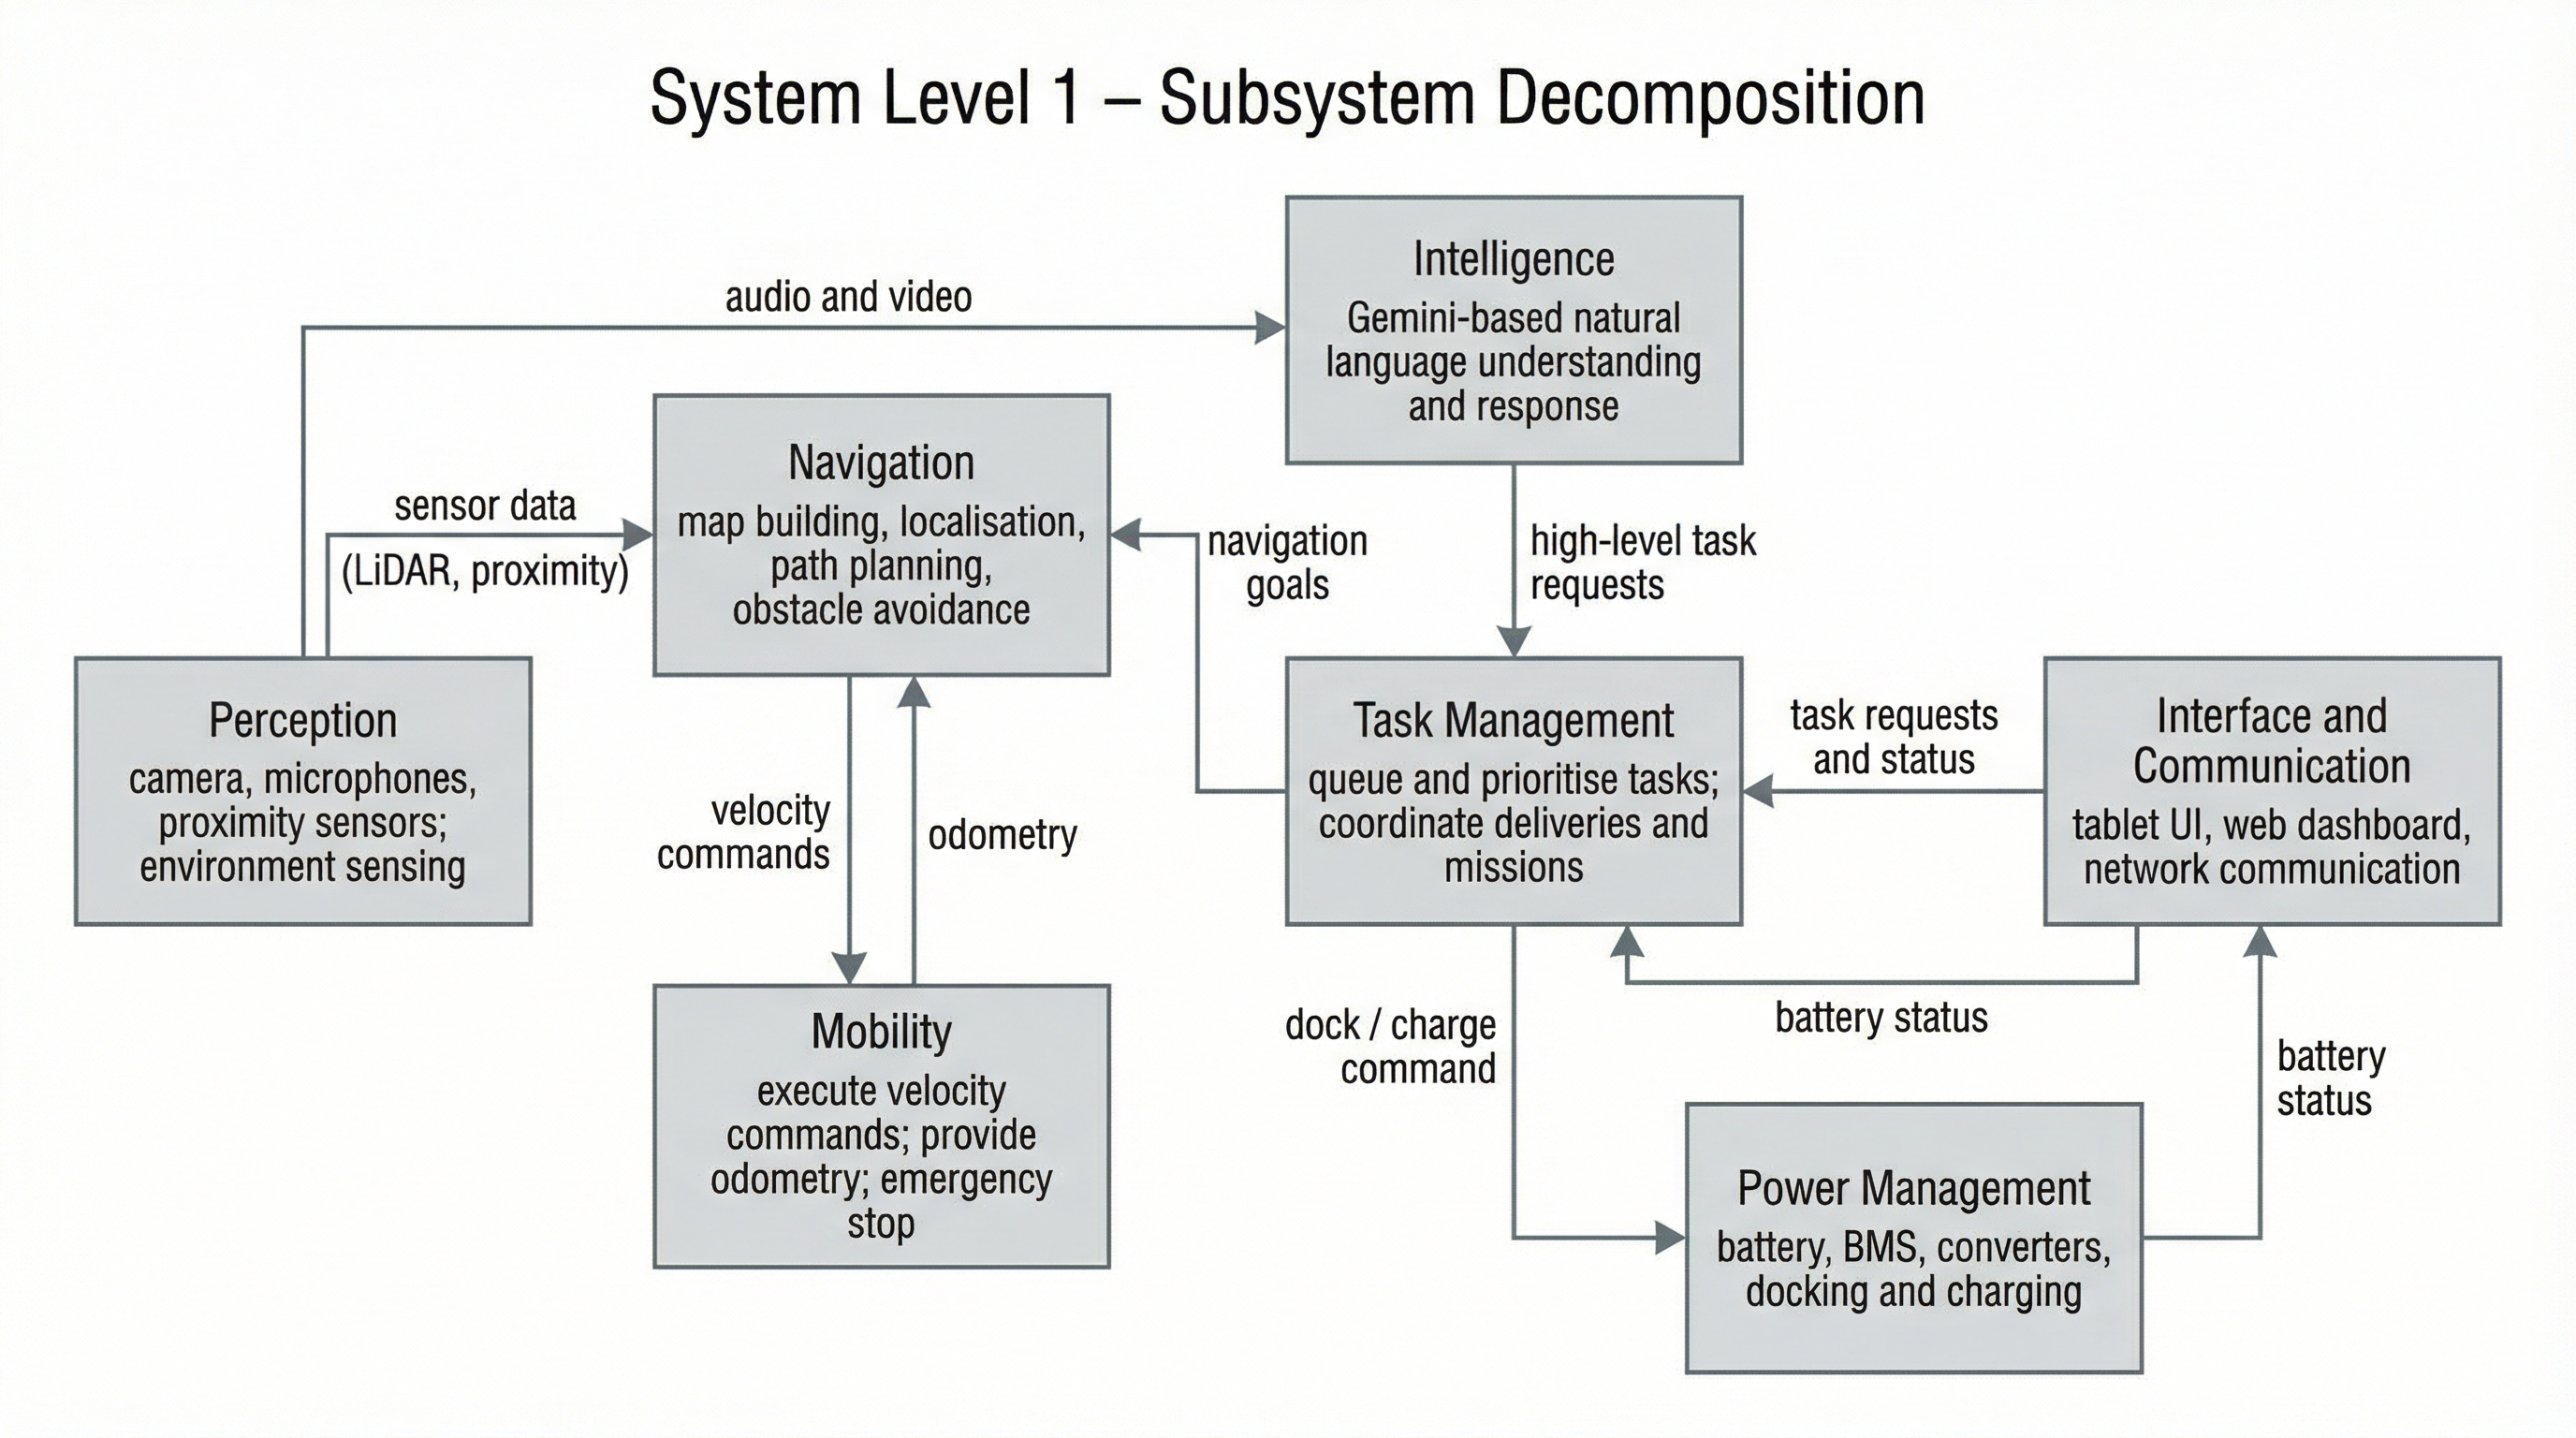
\includegraphics[width=0.95\textwidth]{level1-subsystem-decomposition-1765609443106.png}
    \caption{System Level~1 subsystem decomposition and key data/control flows across the seven subsystems.}
    \label{fig:level1-subsystems}
\end{figure}

% ============================================================
% 5. SYSTEM IMPLEMENTATION  (kept in full - the core contribution)
% ============================================================
\section{System Implementation: Results and Discussion}
\label{sec:implementation}

This section documents the hardware realisation, software development, and validation testing of TAMRA (Task-Agnostic Modular Robotic Apparatus). The first semester established the design foundation. The second semester converted those decisions into a working system and required two course corrections that are explained before the technical content: a platform change, and a scope refinement.

\subsection{Platform Selection: From TurtleBot to iMRP500}

Semester one was spent studying TurtleBot~4 and iCreate~3 in simulation. That work was productive --- it built a solid foundation in ROS~2~\cite{macenski2022ros2}, SLAM, and sensor fusion that carried into implementation. When procurement time arrived, however, both platforms were ruled out.

iRobot, manufacturer of the iCreate~3, entered bankruptcy proceedings at the same time the team needed to commit a purchase~\cite{irobot2024create3}. With a fixed budget and an eight-week deadline, depending on a platform with uncertain long-term support was not viable. TurtleBot~4 shares the same Create~3 base and carries the same risk.

Beyond sustainability, both platforms lack any engineered mounting interface for a body structure --- neither is designed to accept a tall shell, and improvised fixturing would have introduced mechanical instability incompatible with the physical design goals.

This platform transition proved to be a critical turning point. The alternative platforms discovered during the search were superior across every relevant dimension: payload capacity, onboard sensor integration, structural rigidity, and long-term vendor support. The switch was the difference between a system that could be realistically deployed in a service environment and one that would remain a laboratory prototype.

\subsubsection{The Service Robot Landscape}

Before selecting a platform, it was important to understand the broader ecosystem. Service robots divide into two fundamentally different categories: \textbf{ready-to-use robots} pre-configured for a specific industry vertical, and \textbf{chassis bases} that expose a raw navigation and sensor stack for a developer to build upon. Figure~\ref{fig:landscape} maps the ecosystem.

\begin{figure}[H]
\centering
\noindent\textbf{Chassis Bases} \hfill {\small (open platform, developer builds on top)}
\vspace{4pt}

\noindent
\begin{minipage}[t]{0.23\linewidth}\centering
  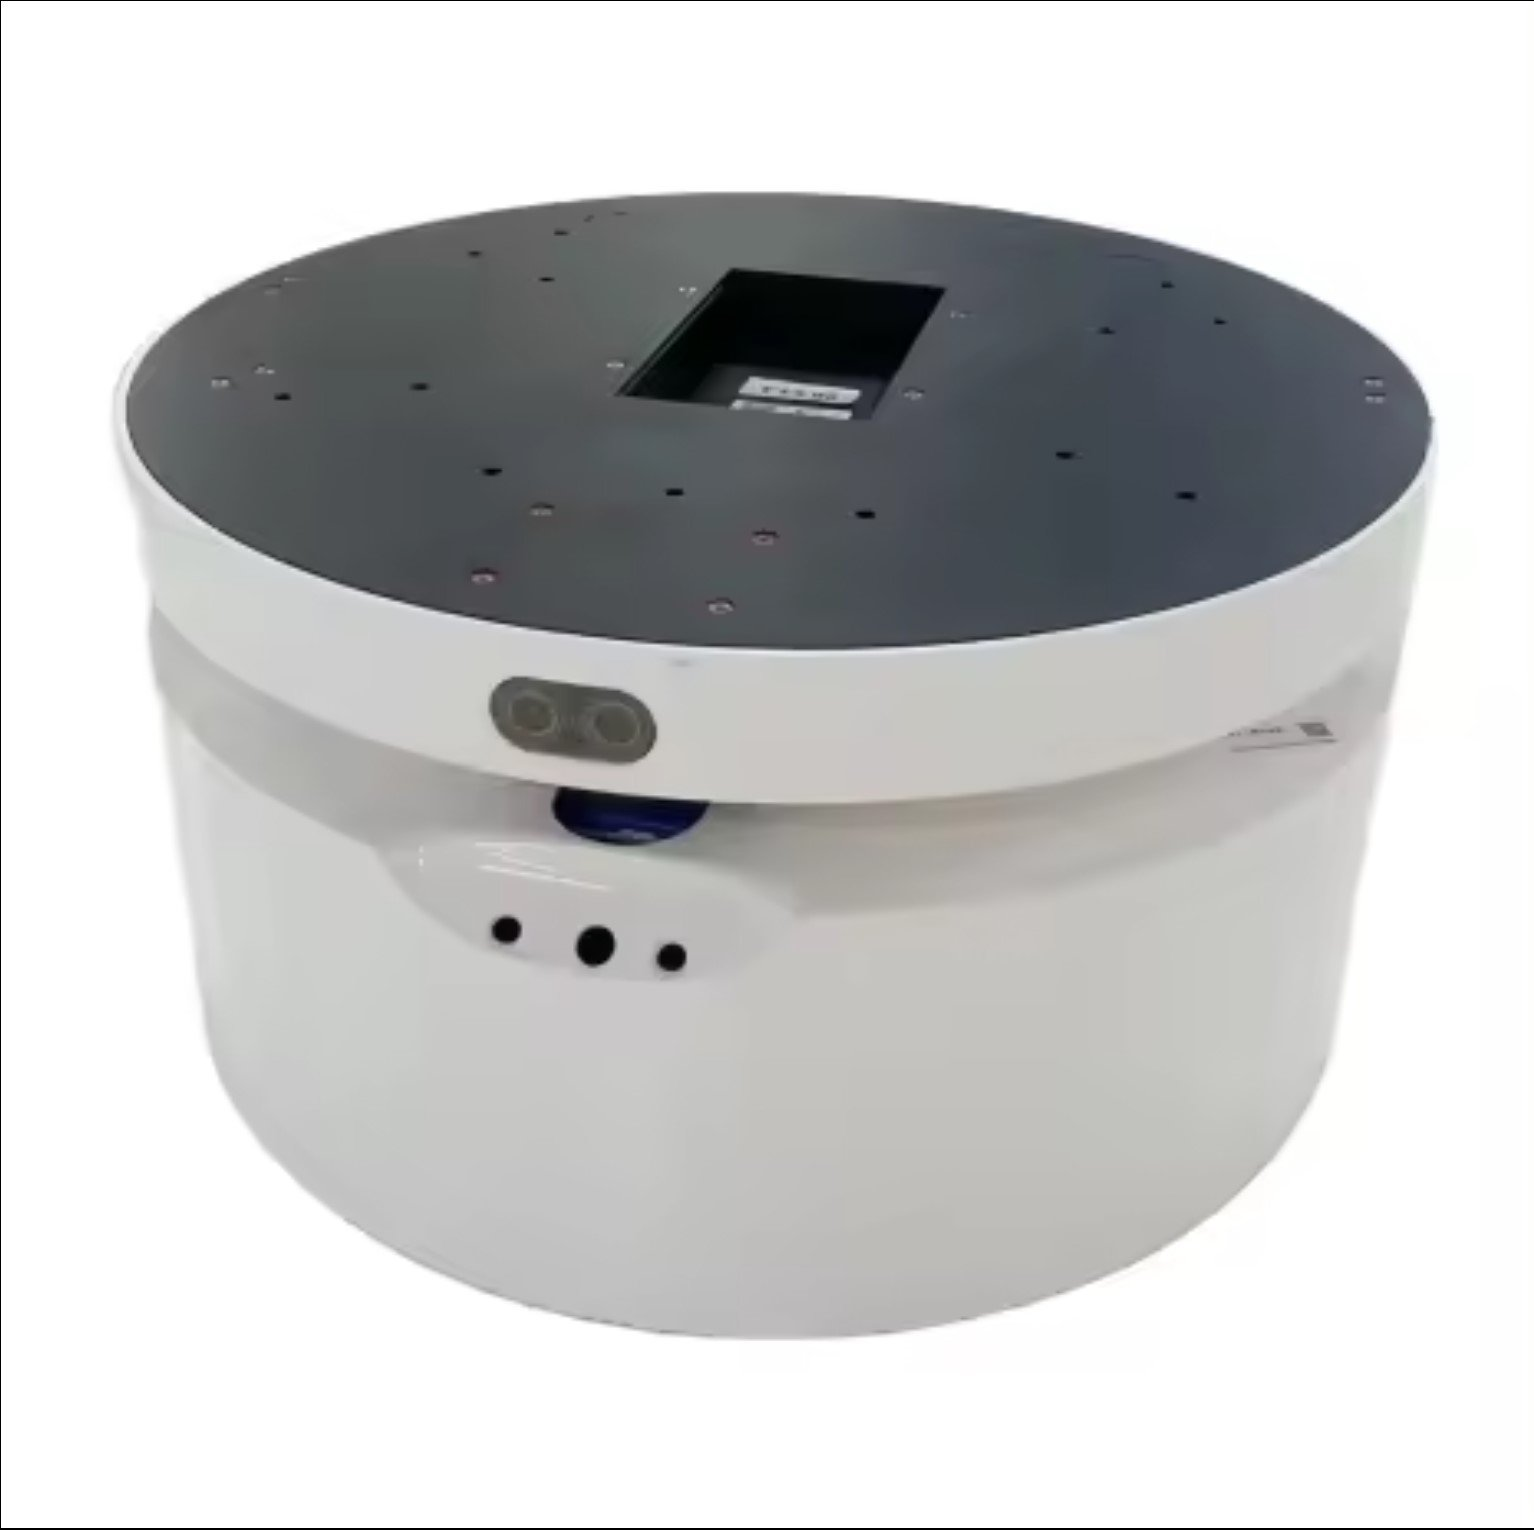
\includegraphics[width=\linewidth,height=3.0cm,keepaspectratio]{plat_ciot.jpg}\\[3pt]
  {\small\textbf{iMRP500}\\ \textit{Selected}\\ 850\,OMR incl.\ shipping}
\end{minipage}\hfill
\begin{minipage}[t]{0.23\linewidth}\centering
  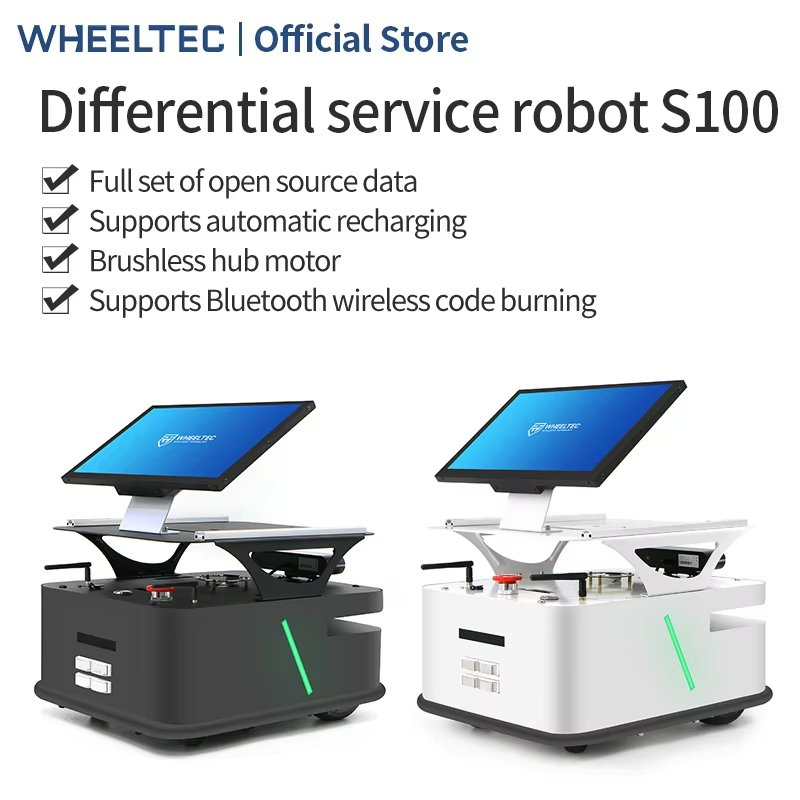
\includegraphics[width=\linewidth,height=3.0cm,keepaspectratio]{plat_wheeltec.jpg}\\[3pt]
  {\small\textbf{Wheeltec S100}\\ \textit{ROS~1/2, academic}\\ from 550\,OMR}
\end{minipage}\hfill
\begin{minipage}[t]{0.23\linewidth}\centering
  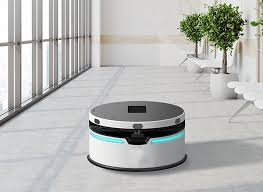
\includegraphics[width=\linewidth,height=3.0cm,keepaspectratio]{plat_waterdrop.jpg}\\[3pt]
  {\small\textbf{Water Drop (Shuidi II)}\\ \textit{Circular, 50\,kg payload}\\ $\sim$\$2{,}285}
\end{minipage}\hfill
\begin{minipage}[t]{0.23\linewidth}\centering
  \vspace{0.6cm}
  {\small\textbf{Slamtec Series}\\ SDP Mini \$500\\ Apollo 2.0\\ Hermes $\sim$\$2{,}000}
\end{minipage}

\vspace{10pt}
\noindent\rule{\linewidth}{0.3pt}
\vspace{6pt}

\noindent\textbf{Ready-to-Use Robots} \hfill {\small (closed software, industry-specific)}
\vspace{4pt}

\noindent
\begin{minipage}[t]{0.23\linewidth}\centering
  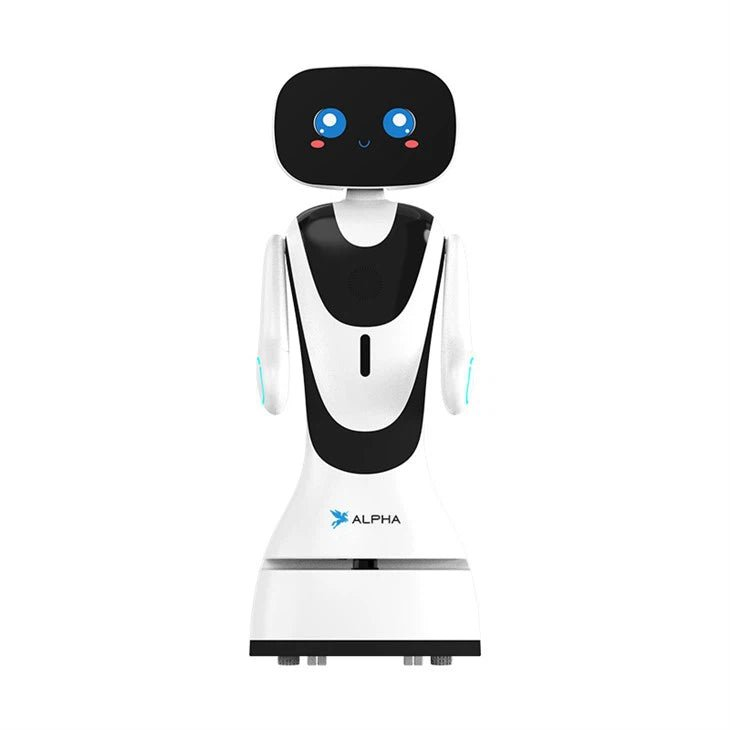
\includegraphics[width=\linewidth,height=3.0cm,keepaspectratio]{plat_reception.jpg}\\[3pt]
  {\small\textbf{Reception / Guide}\\ Touchscreen, face recognition\\ No payload. Guides only.}
\end{minipage}\hfill
\begin{minipage}[t]{0.23\linewidth}\centering
  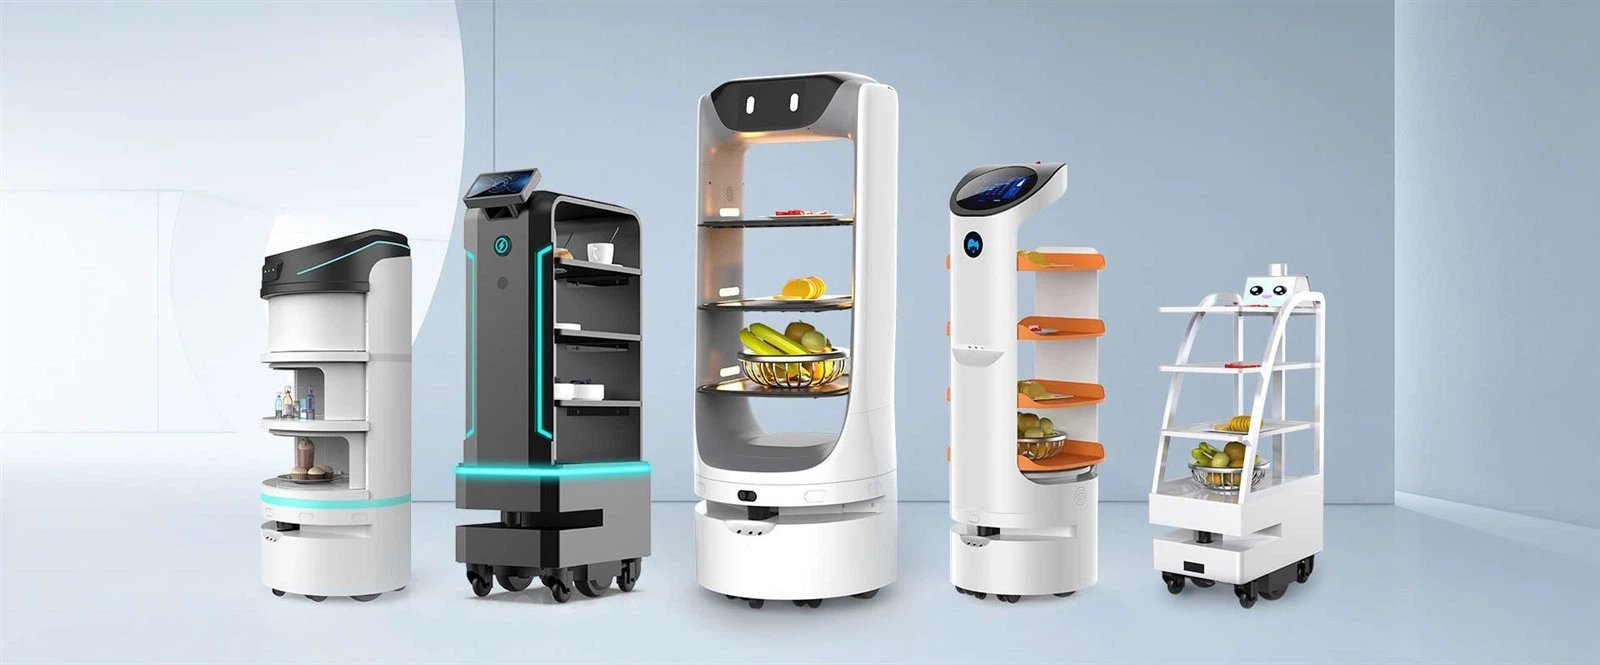
\includegraphics[width=\linewidth,height=3.0cm,keepaspectratio]{plat_restaurant.jpg}\\[3pt]
  {\small\textbf{Restaurant Delivery}\\ e.g.\ Keenon T5\\ Open shelves, \$1{,}700--3{,}000}
\end{minipage}\hfill
\begin{minipage}[t]{0.23\linewidth}\centering
  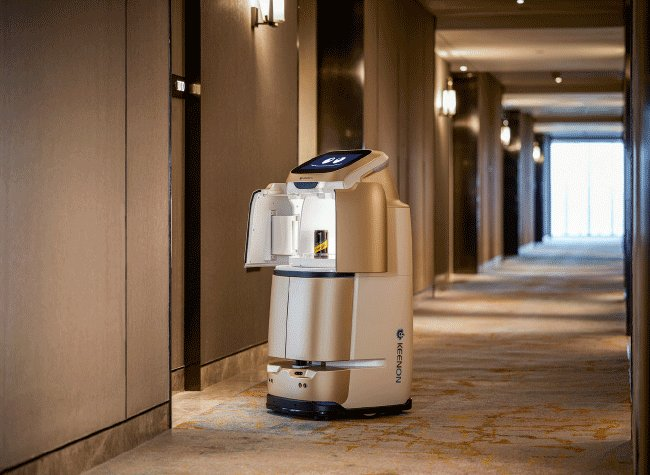
\includegraphics[width=\linewidth,height=3.0cm,keepaspectratio]{plat_hotel.jpg}\\[3pt]
  {\small\textbf{Hotel Delivery}\\ Enclosed locking compartments\\ PIN/QR access, elevator control}
\end{minipage}\hfill
\begin{minipage}[t]{0.23\linewidth}\centering
  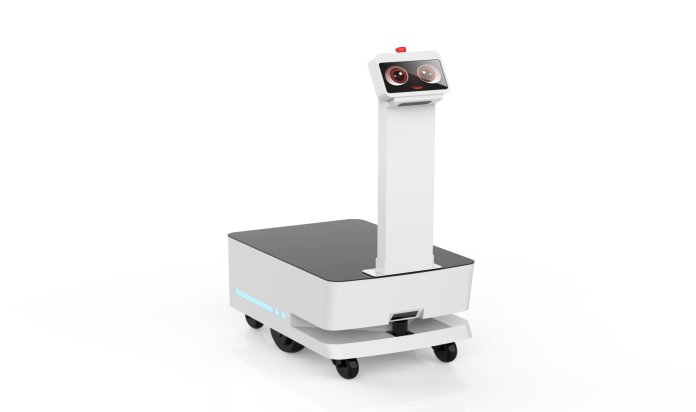
\includegraphics[width=\linewidth,height=3.0cm,keepaspectratio]{plat_factory.jpg}\\[3pt]
  {\small\textbf{Factory AMRs}\\ 100--1{,}000+\,kg payload\\ Pallet lift, tow carts}
\end{minipage}

\caption{Service robot ecosystem. \textit{Top row}: chassis bases that expose open navigation APIs for developers to build on. \textit{Bottom row}: ready-to-use robots locked to a single industry vertical. None of the ready-to-use categories offer an open interface for adding conversational AI, custom bodies, or research-level sensor access --- hence the chassis-base approach.}
\label{fig:landscape}
\end{figure}

\noindent The ready-to-use categories each serve a narrow purpose. Restaurant robots use open shelves optimised for kitchen-to-table trips. Hotel robots carry enclosed locking compartments that only the correct guest can open via PIN or QR code, and can coordinate with elevators. Reception robots are screen-focused and carry no payload. None matched the requirement for a single platform combining autonomous navigation, conversational AI, item delivery, and telepresence at research-accessible cost. Chassis bases expose raw navigation and sensor data for a developer to build upon; six were evaluated in depth.

\subsubsection{Comparative Platform Evaluation}

Table~\ref{tab:platform_eval} summarises the six chassis platforms reviewed through vendor documentation, ROS compatibility, payload ratings, sensor suites, and structural mounting options.

\begin{table}[H]
\centering
\small
\caption{Mobile chassis platforms evaluated for TAMRA.}
\label{tab:platform_eval}
\setlength{\tabcolsep}{4pt}
\begin{tabular}{@{} >{\raggedright\arraybackslash}p{2.8cm} r >{\raggedright\arraybackslash}p{1.5cm} >{\raggedright\arraybackslash}p{3.4cm} @{}}
\toprule
\textbf{Platform} & \textbf{USD} & \textbf{Payload} & \textbf{Verdict} \\
\midrule
Bao Xiaomi Mini    & 2{,}000 & Service only & Consumer-grade; no payload; closed nav \\
Reeman Moon Knight & 2{,}380 & 60\,kg       & Android SDK; limited open ROS support \\
\textbf{iMRP500}   & \textbf{1{,}550} & \textbf{50\,kg} & \textbf{Selected (AHP score 6.76)} \\
Wheeltec S100      & 1{,}250 & $\sim$15\,kg & Low payload; ROS~1 only; academic focus \\
Timo AI Robot      & 2{,}500 & Service only & Proprietary nav API; no raw data access \\
Uwant T5/T6        & 1{,}700 & 40\,kg       & Closed SLAM; no raw sensor access \\
\bottomrule
\end{tabular}
\end{table}

\noindent The iMRP500 scored highest under the AHP criteria established in Section~\ref{sec:design} (Reliability~47\%, Development~Speed~30\%, Cost~15\%, Customisability~8\%). It was the only platform that combined a 50\,kg payload, an integrated industrial sensor suite with raw data accessible over a documented WebSocket protocol, and a circular footprint with structural mounting points for the body shell.

Before committing, the capability gap between TAMRA and the commercial hospital robots it is meant to compete with was assessed. Table~\ref{tab:commercial_comparison} shows where existing platforms fall short.

\begin{table}[H]
\centering
\small
\caption{Capability comparison with commercial hospital service robots.}
\label{tab:commercial_comparison}
\setlength{\tabcolsep}{4pt}
\begin{tabular}{@{} l c c c c r @{}}
\toprule
 & \textbf{Nav} & \textbf{Delivery} & \textbf{Voice AI} & \textbf{Telepres.} & \textbf{Price} \\
\midrule
PuduBot~2 \cite{pudubot2}          & \checkmark & \checkmark & --         & --         & \$12{,}000 \\
Keenon M2 \cite{m2medical}         & \checkmark & \checkmark & --         & --         & \$47{,}500 \\
Peanut Medical \cite{peanutmedical}& \checkmark & \checkmark & --         & \checkmark & \$12{,}700 \\
PUDU CC1 \cite{puducc1}            & \checkmark & --         & --         & --         & \$16{,}800 \\
\textbf{TAMRA}                     & \checkmark & \checkmark & \checkmark & \checkmark & \textbf{\$3{,}200} \\
\bottomrule
\end{tabular}
\end{table}

\subsection{Hardware Implementation}

\subsubsection{iMRP500 Chassis}

The iMRP500 is a circular differential-drive industrial chassis, 500\,mm in diameter, whose key specifications are given in Table~\ref{tab:imrp500_spec}. Procurement cost including shipping was 850\,OMR.

\begin{table}[H]
\centering
\small
\caption{iMRP500 chassis specifications.}
\label{tab:imrp500_spec}
\setlength{\tabcolsep}{5pt}
\begin{tabular}{@{} >{\raggedright\arraybackslash}p{3.8cm} >{\raggedright\arraybackslash}p{4.2cm} @{}}
\toprule
\textbf{Parameter} & \textbf{Value} \\
\midrule
Diameter / height      & 500\,mm / 310\,mm \\
Maximum payload        & 50\,kg \\
Drive                  & 2 servo hub motors, 5 wheels \\
LiDAR                  & TOF, 360$^{\circ}$, 20\,m range \\
Depth camera           & RGBD structured-light, 0.6--8\,m \\
IMU                    & 6-axis \\
Battery                & 24\,V / 20\,Ah Li-ion \\
Runtime (no load)      & 12\,h \\
Navigation accuracy    & $\pm$5\,cm \\
Max navigation speed   & 0.8\,m/s \\
Onboard compute        & Off-shelf SoC, Ubuntu 20.04 \\
Communication          & WebSocket port~9090, MJPEG port~9099 \\
Safety                 & Hardware E-stop (ISO~13850), soft-stop service \\
\bottomrule
\end{tabular}
\end{table}

\paragraph{Reverse-engineering the communication layer.}
The chassis ships with a proprietary operator application and a Chinese-language protocol document. Commissioning it for research required mapping the full ROS topic and service graph over the WebSocket bridge. The following sensor topics were confirmed and integrated:

\begin{itemize}
  \item \texttt{/scan} --- 360$^{\circ}$ TOF LiDAR scan, primary localisation input
  \item \texttt{/upcamera/rgb/image\_raw} and \texttt{/upcamera/depth/image\_raw} --- RGBD camera mounted pointing upward to detect overhead obstacles (counter overhangs, low tables)
  \item \texttt{/robot\_pose} --- fused position estimate $(x,\,y,\,\theta)$
  \item \texttt{/robot\_status} --- battery percentage, charger state, navigation status code
  \item \texttt{/mobile\_base/sensors/core} --- wheel encoder odometry, ultrasonic proximity (3-point frontal)
  \item \texttt{/localization\_confidence} --- real-time localisation quality score (0.0--1.0)
\end{itemize}

\noindent Navigation goals are dispatched via the \texttt{/poi} service using named waypoints stored in the chassis map database. The navigation stack is built on Nav2~\cite{macenski2023nav2}. The localisation stack fuses three complementary sources. Let $\mathbf{x}_t = [x,\,y,\,\theta]^T$ be the robot pose at time $t$. An extended Kalman filter~\cite{thrun2005probabilistic} operates in two steps:
\begin{align}
  \textit{Predict:}\quad & \hat{\mathbf{x}}_{t}^{-} = f(\mathbf{x}_{t-1},\,\mathbf{u}_t) \\[4pt]
  \textit{Update:}\quad  & \hat{\mathbf{x}}_{t} = \hat{\mathbf{x}}_{t}^{-}
    + \mathbf{K}_t\!\left(\mathbf{z}_t^{\text{LiDAR}} - h\!\left(\hat{\mathbf{x}}_{t}^{-}\right)\right)
\end{align}
where $\mathbf{u}_t$ encodes wheel encoder and IMU data, $\mathbf{z}_t^{\text{LiDAR}}$ is the scan-match observation, $h(\cdot)$ is the observation model, and $\mathbf{K}_t$ is the Kalman gain. The costmap runs four stacked layers: a LiDAR obstacle layer (4\,m range, 0.6\,m max height), an upward-camera layer for overhead detection (3.5\,m range, 2\,m max height), a downward-camera layer, and an inflation layer (0.8\,m radius, scaling factor~10). The local costmap updates at 8\,Hz over a $3\times3$\,m window at 0.03\,m resolution; the global costmap at 4\,Hz over $10\times10$\,m at 0.05\,m resolution.

\paragraph{Internal architecture.}
Physical inspection of the chassis electronics revealed how the manufacturer achieved its cost point. Three layers are present: the bottom layer uses commodity CNC stepper motor drivers (identifiable by their green terminal blocks and PWR/ALM LED indicators); the mid layer is an off-the-shelf SoC board with USB and Ethernet ports; the top layer uses sensor interface boards from the 3D-printer ecosystem. The drive motors are hub motors from the electric scooter supply chain. This architecture substitutes widely available commodity components for custom ASICs, reducing cost without sacrificing reliability at service-robot duty cycles.

\begin{figure}[H]
  \centering
  \begin{minipage}[t]{0.48\linewidth}\centering
    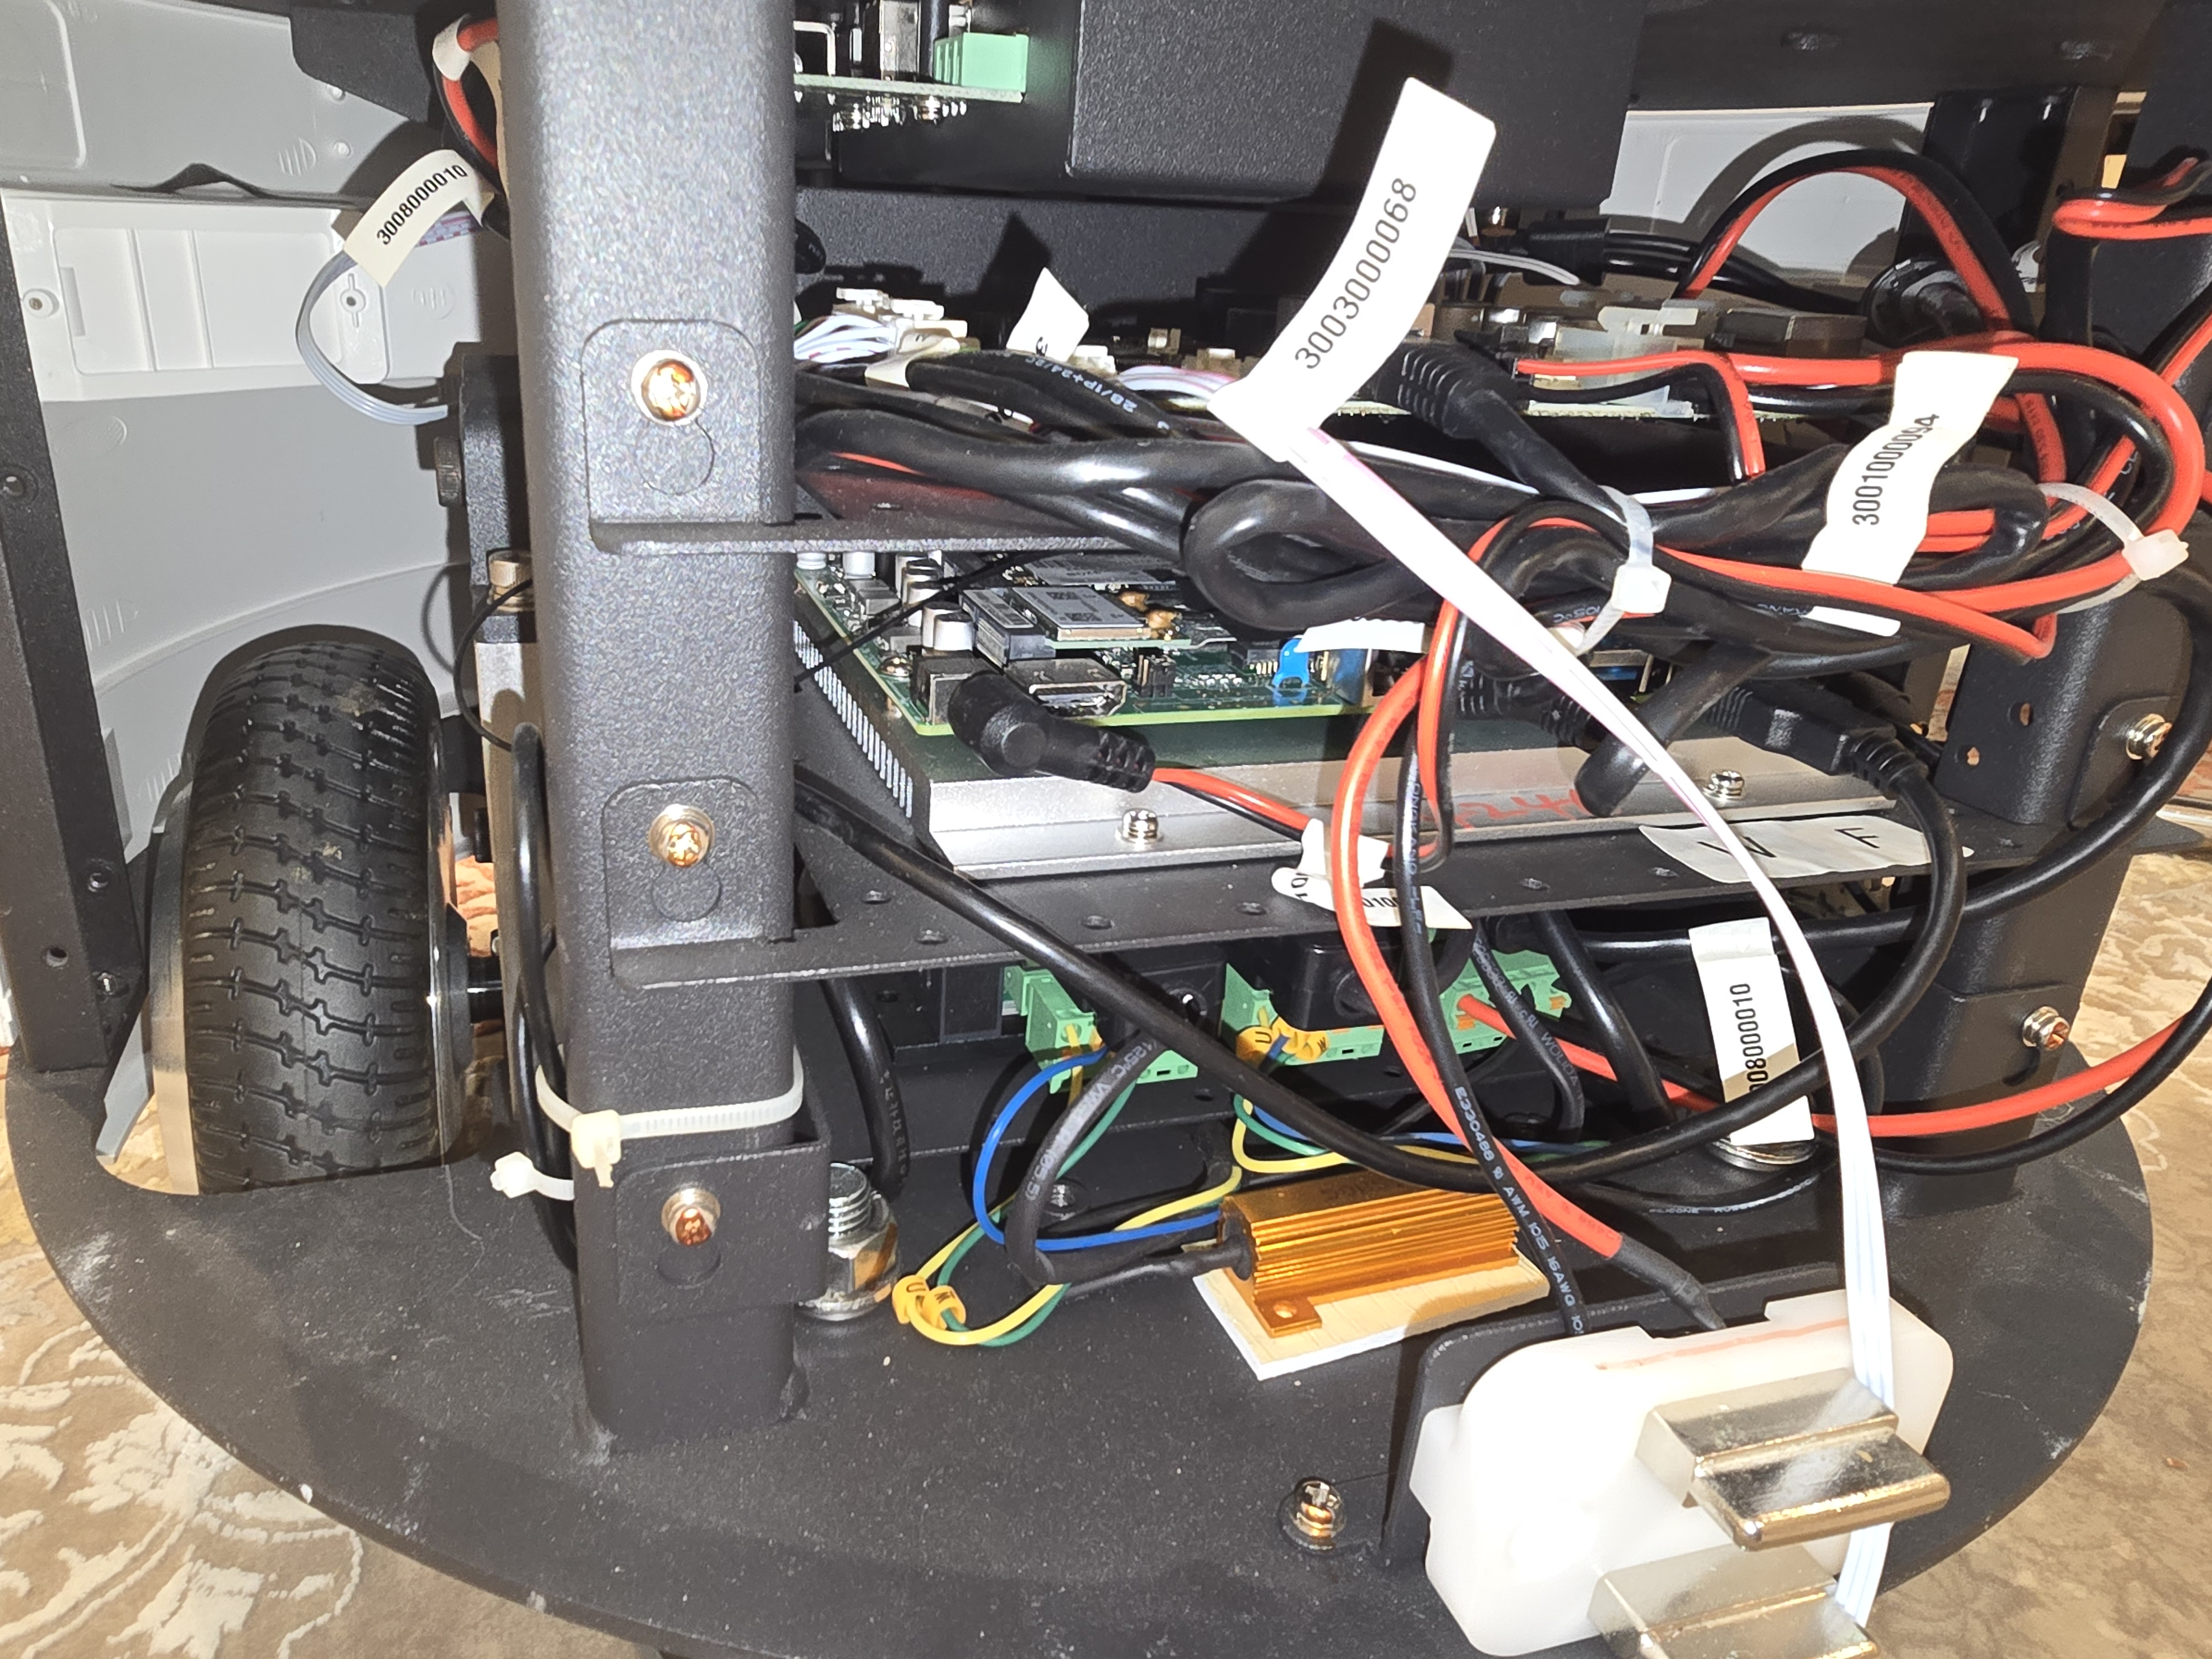
\includegraphics[width=\linewidth,height=5.5cm,keepaspectratio]{internals1.jpeg}
  \end{minipage}\hfill
  \begin{minipage}[t]{0.48\linewidth}\centering
    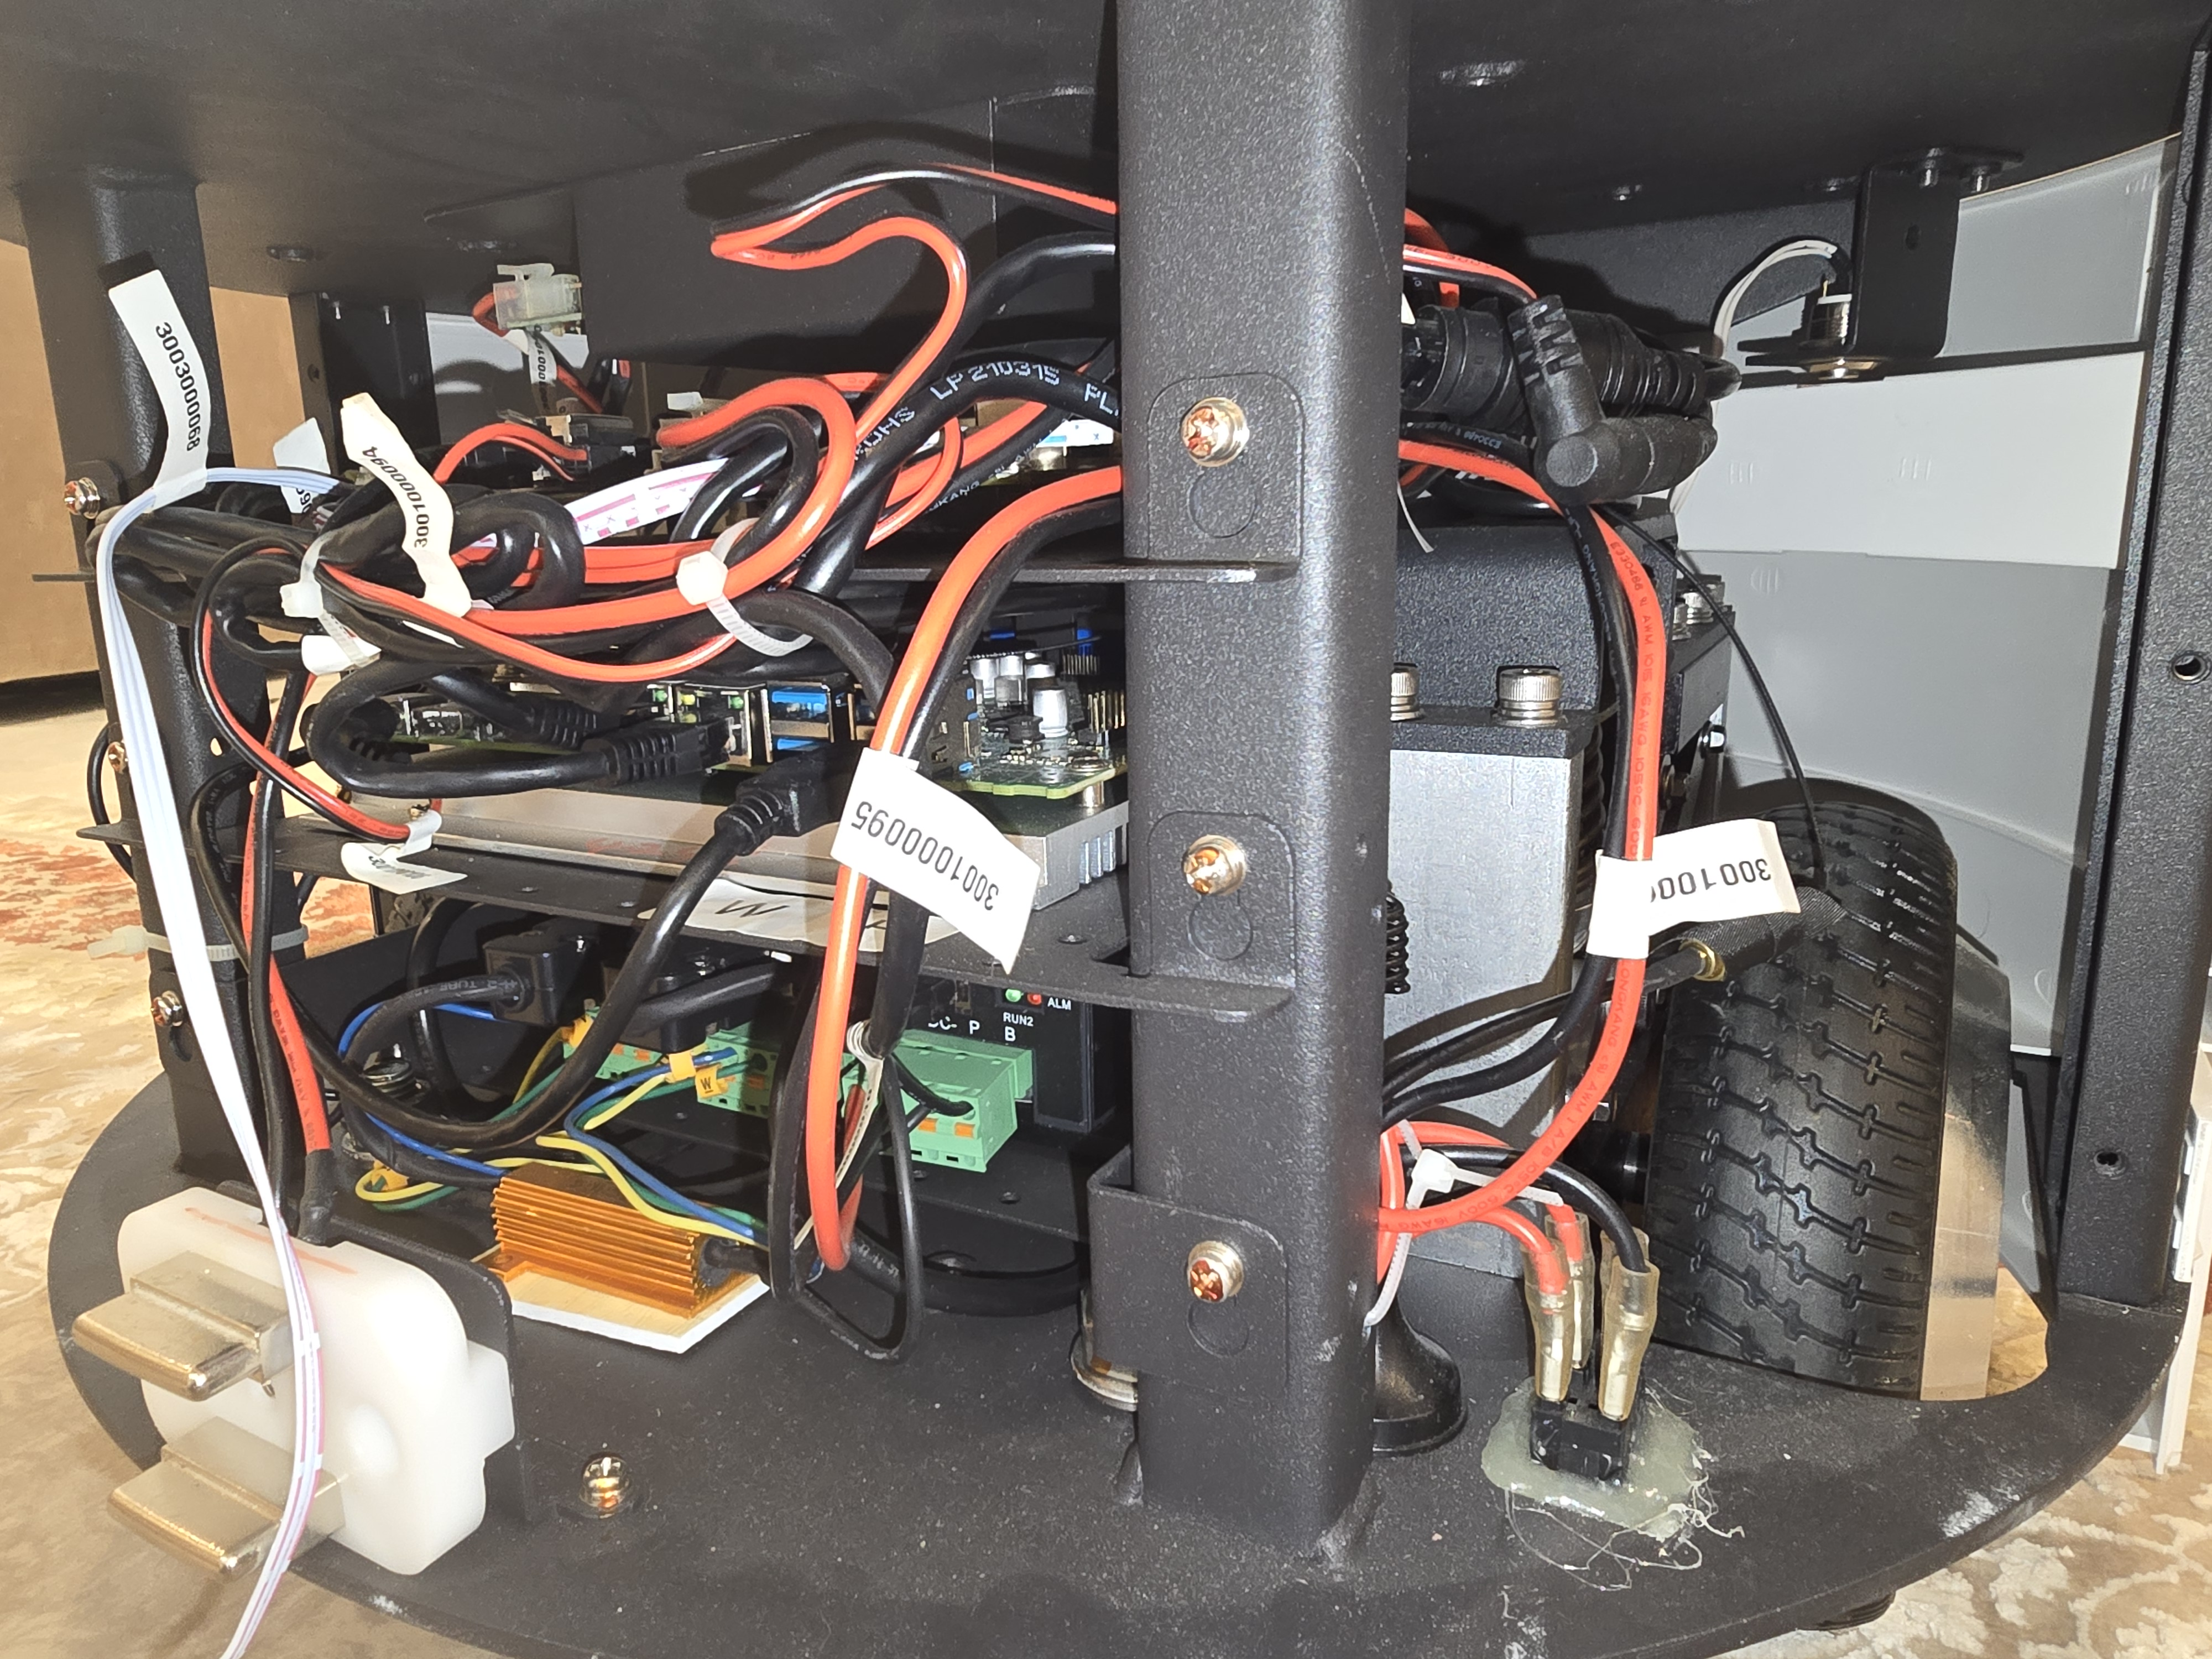
\includegraphics[width=\linewidth,height=5.5cm,keepaspectratio]{internals2.jpeg}
  \end{minipage}
  \caption{iMRP500 internal electronics: commodity CNC stepper drivers, off-the-shelf SoC, and 3D-printer-style sensor boards. Scooter hub motors are visible at the periphery.}
  \label{fig:internals}
\end{figure}

\subsubsection{Body Shell Design and Fabrication}

The body shell connects the 500\,mm circular chassis to the robot's human-facing components: the display, the storage compartment, and the exterior surface that users interact with. Eleven functional requirements constrained the design:

\begin{itemize}
  \item Display tilted at 40$^{\circ}$ from horizontal for ergonomic use at standing and seated heights~\cite{frontiers2024}
  \item Display recess accepting a future larger screen without structural change (5\,mm step, $360\times260$\,mm outer frame)
  \item Internal tray for secure transport; external storage compartment for accessible delivery
  \item Footprint within the 500\,mm chassis diameter (LiDAR clearance requirement)
  \item Added mass not exceeding 12\,kg (chassis centre-of-mass stability limit)
  \item Total height not exceeding 1{,}100\,mm (tipping stability per chassis datasheet)
  \item Hospital-compatible materials: no sharp edges, surfaces compatible with standard disinfectant protocols~\cite{intel2024}
  \item Concealed cable routing between tablet, display driver, and chassis
  \item Manufacturable locally using available trades
  \item Budget not exceeding 300\,OMR
  \item Warm, approachable aesthetic to reduce patient anxiety~\cite{beran2013}
\end{itemize}

\paragraph{Design workflow.}
The shell was developed in three stages. First, concept rendering was used to rapidly explore aesthetic directions. Hundreds of configurations were reviewed within hours --- far faster than equivalent CAD iteration --- converging on a tapered silhouette with a central wood-veneer accent panel, a recessed display at the top, and a rear storage compartment.

Second, the selected concept image was fed into an AI-based 3D mesh generator (Hunyuan3D~v3.1), producing an initial mesh that captured the organic curvature but contained fabrication-incompatible geometry: overhangs beyond the 500\,mm radius and incorrect storage proportions.

Third, the mesh was used as a geometric reference for parametric reconstruction in Autodesk Fusion~360, producing fabrication-ready engineering drawings with tolerances. Final dimensions: 900\,mm total height, 500\,mm base (chassis interface), 400\,mm waist, 210\,mm storage depth, 40$^{\circ}$ display tilt.

\begin{figure}[H]
  \centering
  \begin{minipage}[t]{0.36\linewidth}\centering
    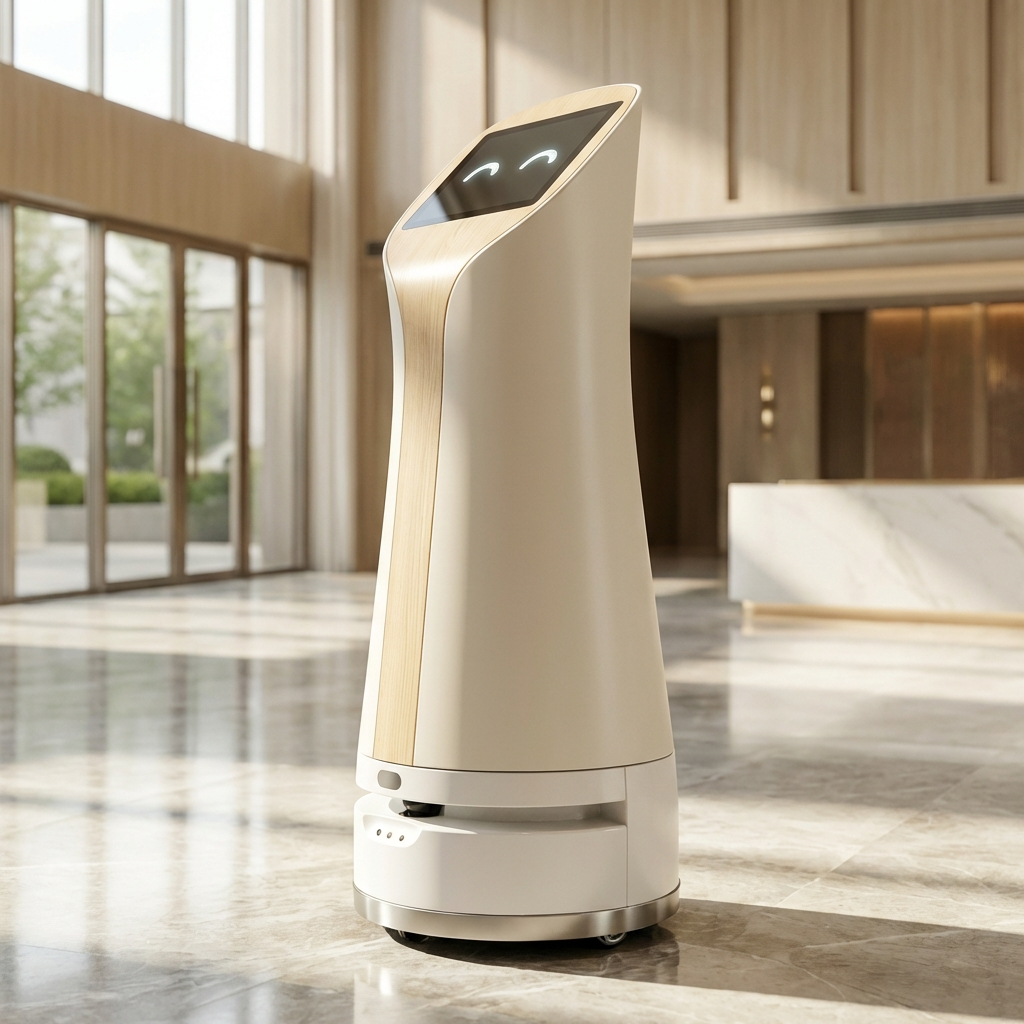
\includegraphics[width=\linewidth]{render_front.jpeg}
    \caption*{(a) Concept render}
  \end{minipage}\hfill
  \begin{minipage}[t]{0.60\linewidth}\centering
    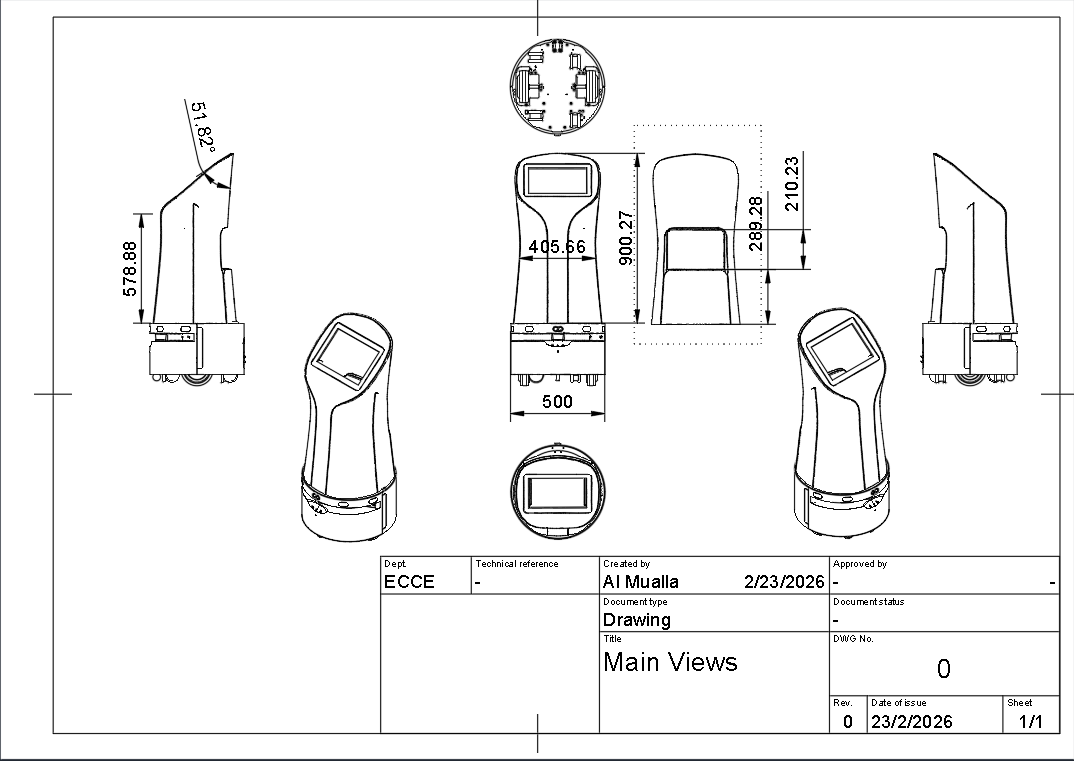
\includegraphics[width=\linewidth]{engn_drawing_robot_dimensions.png}
    \caption*{(b) Fusion~360 engineering drawing}
  \end{minipage}
  \caption{Body shell design workflow: concept render (left) and parametric engineering drawing with fabrication dimensions (right). The 500\,mm base diameter matches the chassis footprint exactly, preserving LiDAR clearance on all sides.}
  \label{fig:design_to_drawing}
\end{figure}

\paragraph{Material selection.}
Several manufacturing routes were evaluated:

\begin{itemize}
  \item \textbf{3D printing} --- rejected: cost-prohibitive for large curved panels, slow for the timeline.
  \item \textbf{Fibreglass composite layup} --- viable but requires specialist skills not locally available at reasonable cost.
  \item \textbf{CNC-machined foam} --- explored seriously. High-density polyurethane foam, when CNC-machined and finished, produces complex curved surfaces visually indistinguishable from moulded plastic or fibreglass, a technique widely used in film-set construction and commercial display fabrication. A local foam artist was consulted, and the result quality was high (Figure~\ref{fig:foam}); however, materials and machining costs reached approximately 400\,OMR, exceeding the body-shell budget, and the option was set aside.
  \item \textbf{MDF with oak veneer} --- selected: widely available, shaped by local carpenters, lightweight, and finishing to a warm surface compatible with clinical-grade disinfectant wipes.
  \item \textbf{Acrylic sheet} --- selected for the display surround: dimensionally precise, smooth, and cleanable.
\end{itemize}

\begin{figure}[H]
  \centering
  \begin{minipage}[t]{0.48\linewidth}\centering
    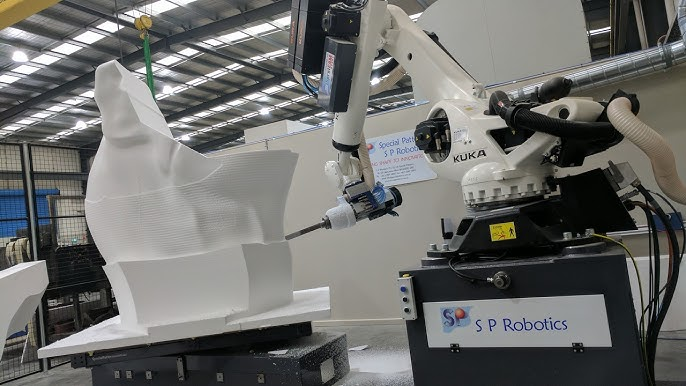
\includegraphics[width=\linewidth,height=5cm,keepaspectratio]{foam_cnc.jpg}
    \caption*{(a) CNC machining of polyurethane foam}
  \end{minipage}\hfill
  \begin{minipage}[t]{0.48\linewidth}\centering
    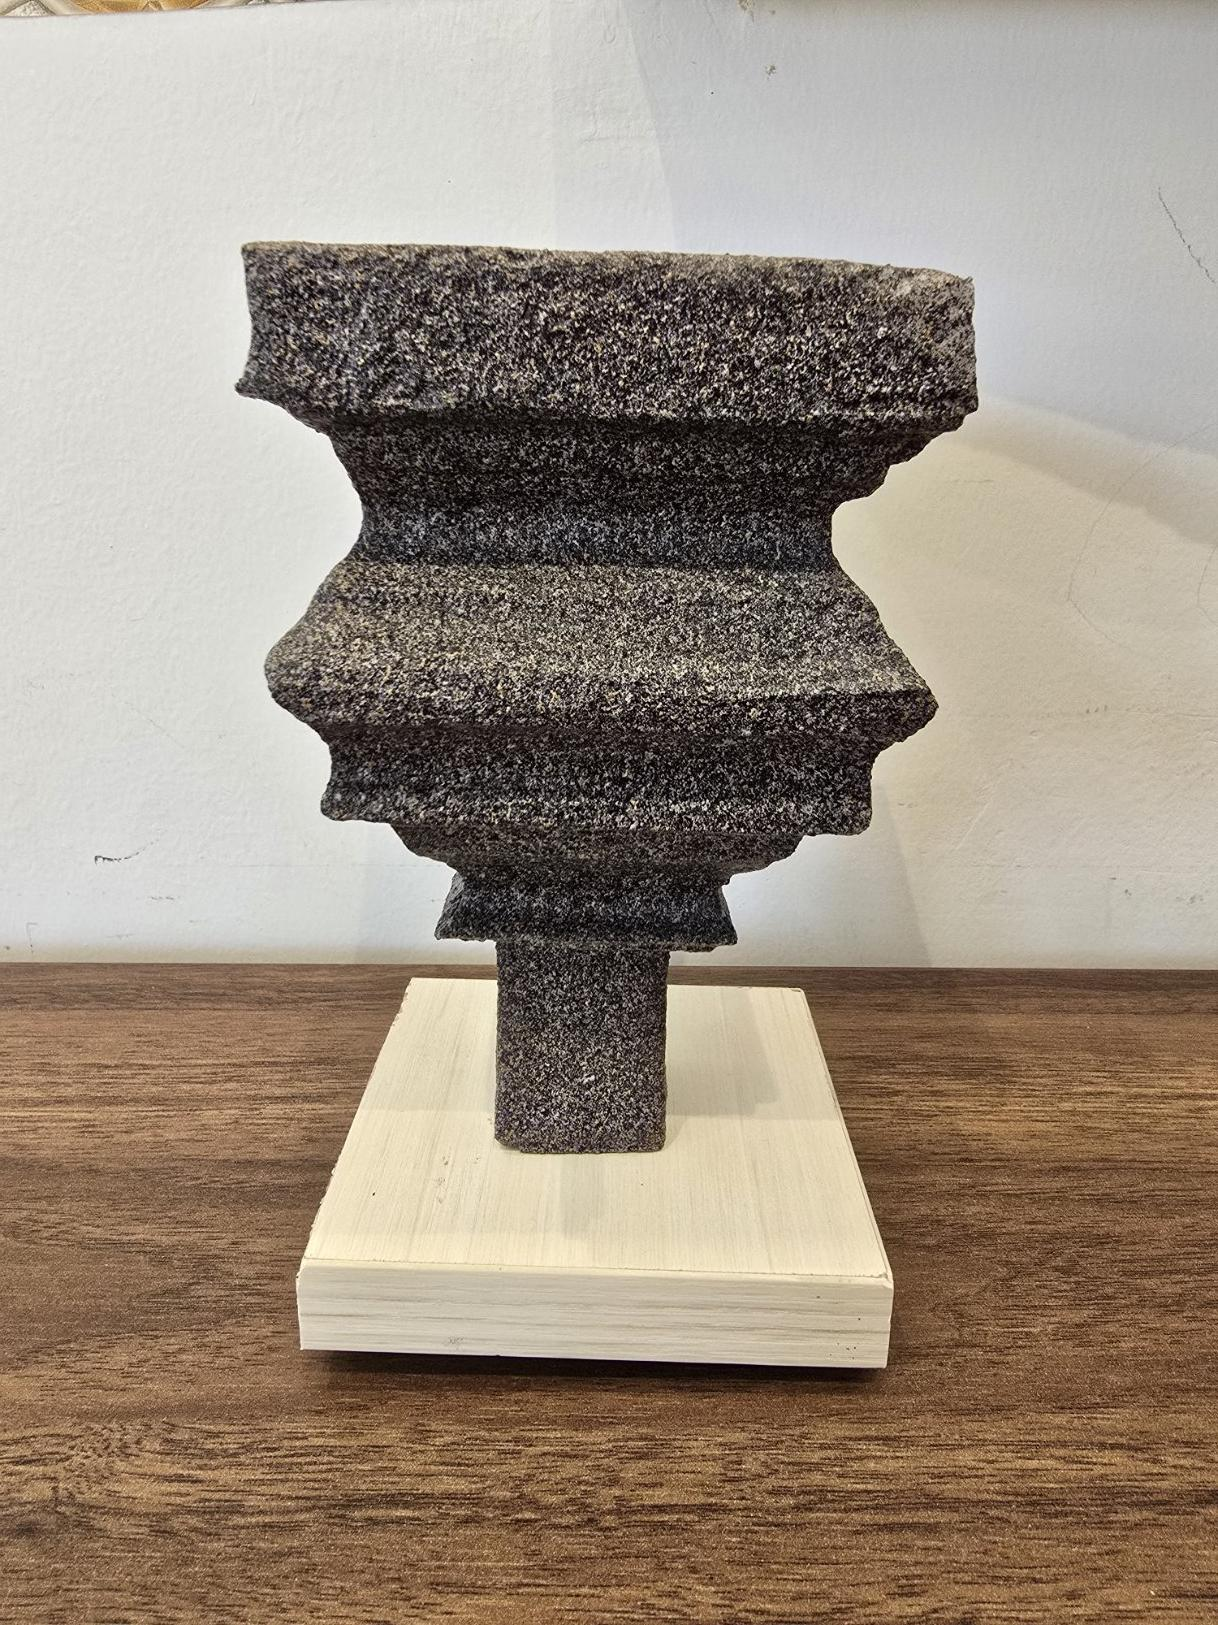
\includegraphics[width=\linewidth,height=5cm,keepaspectratio]{foam_sample.jpg}
    \caption*{(b) Foam test sculpture (material study)}
  \end{minipage}
  \caption{CNC-machined polyurethane foam: the technique produces surfaces indistinguishable from moulded plastic or fibreglass and was explored as a body-shell option. Material and machining costs ($\approx$400\,OMR) placed it above the body-shell budget.}
  \label{fig:foam}
\end{figure}

\paragraph{Fabrication sequence.}
The MDF subframe was cut and assembled at a local carpentry workshop. Figures~\ref{fig:fab_sequence} and~\ref{fig:final_robot} document the process from skeleton to finished robot.

\begin{figure}[H]
  \centering
  \begin{minipage}[t]{0.32\linewidth}\centering
    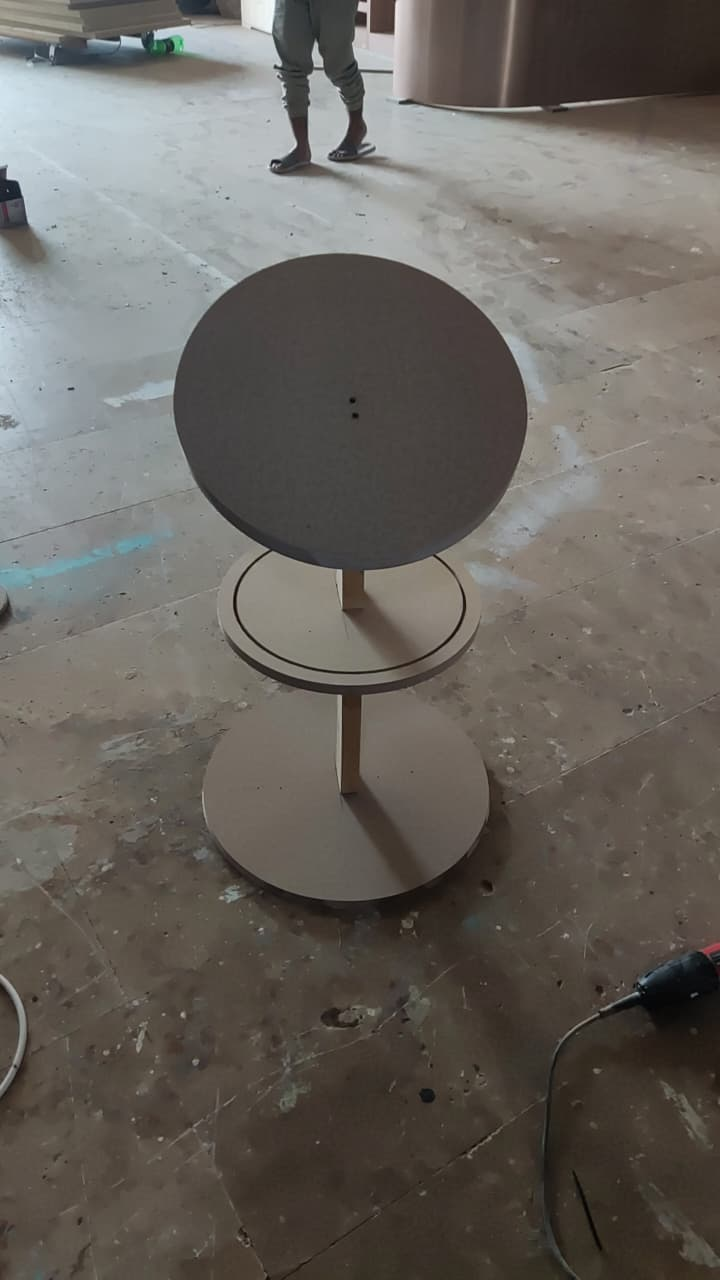
\includegraphics[width=\linewidth,height=5cm,keepaspectratio]{fab_step1.jpeg}
    \caption*{(a) MDF circular decks (skeleton)}
  \end{minipage}\hfill
  \begin{minipage}[t]{0.32\linewidth}\centering
    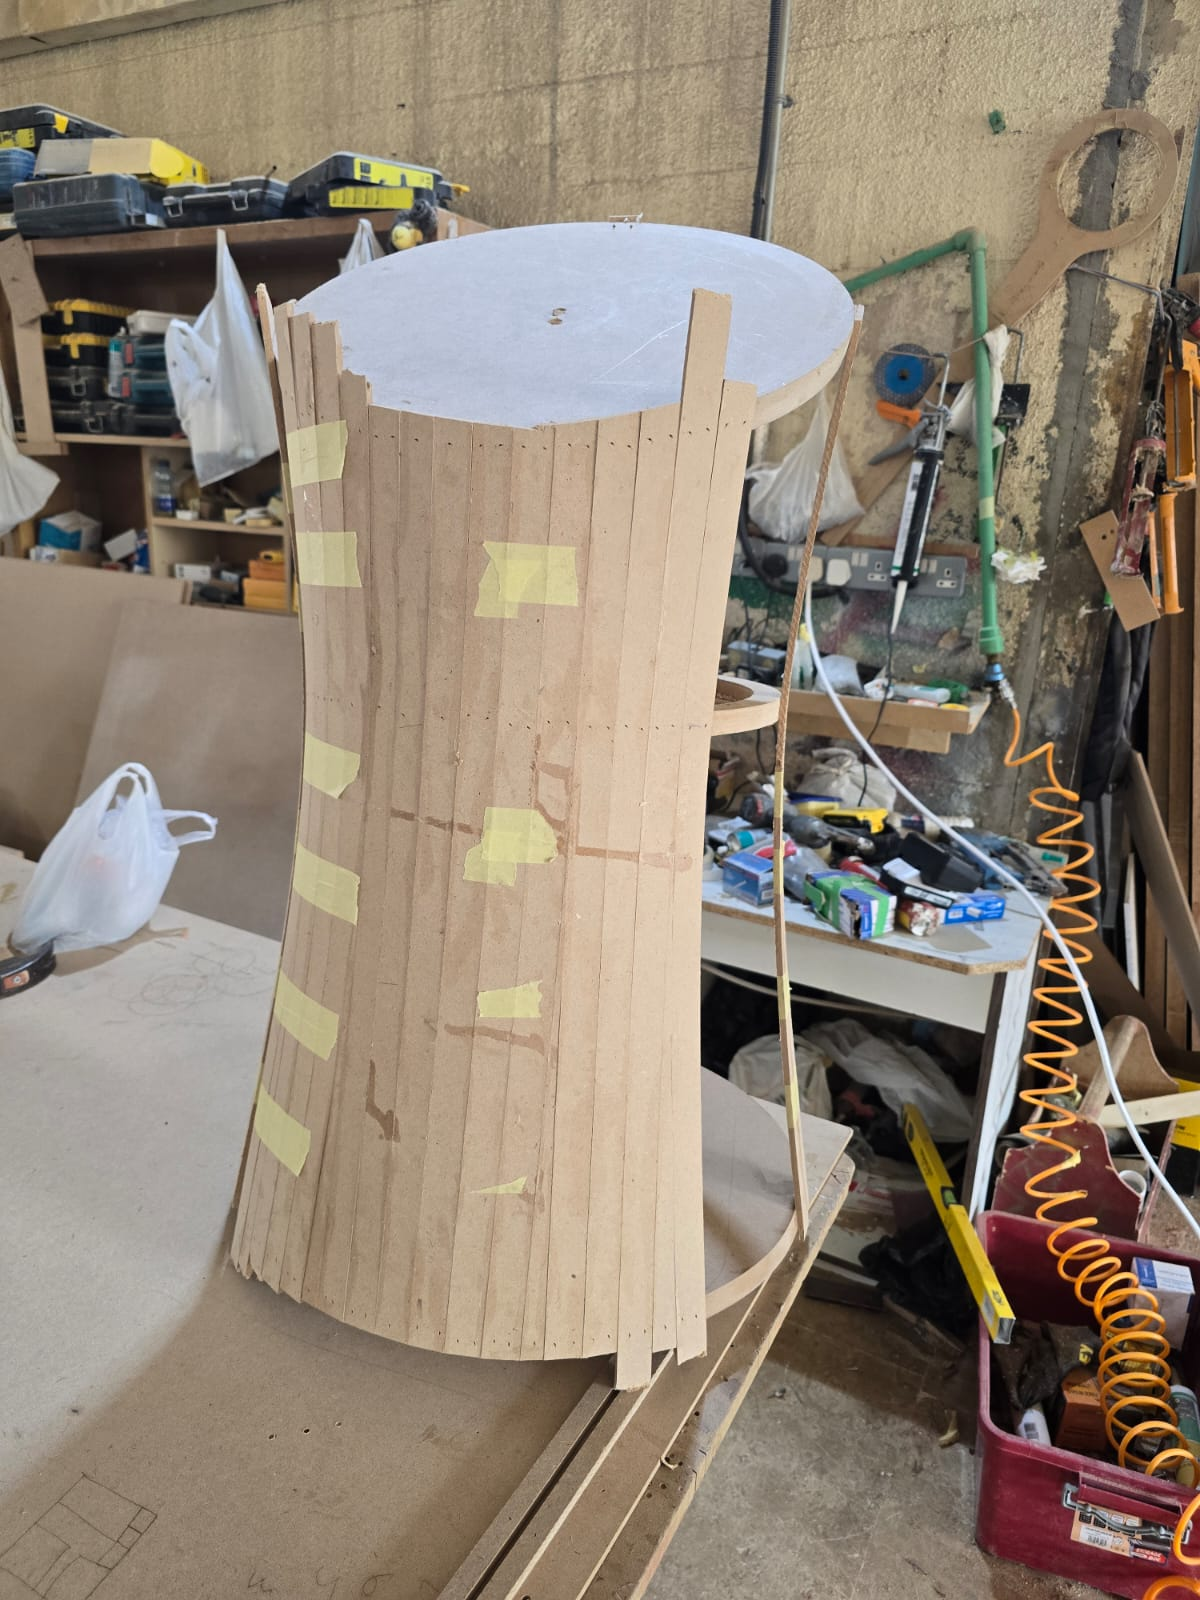
\includegraphics[width=\linewidth,height=5cm,keepaspectratio]{fab_step3.jpeg}
    \caption*{(b) Laminated bent MDF strips}
  \end{minipage}\hfill
  \begin{minipage}[t]{0.32\linewidth}\centering
    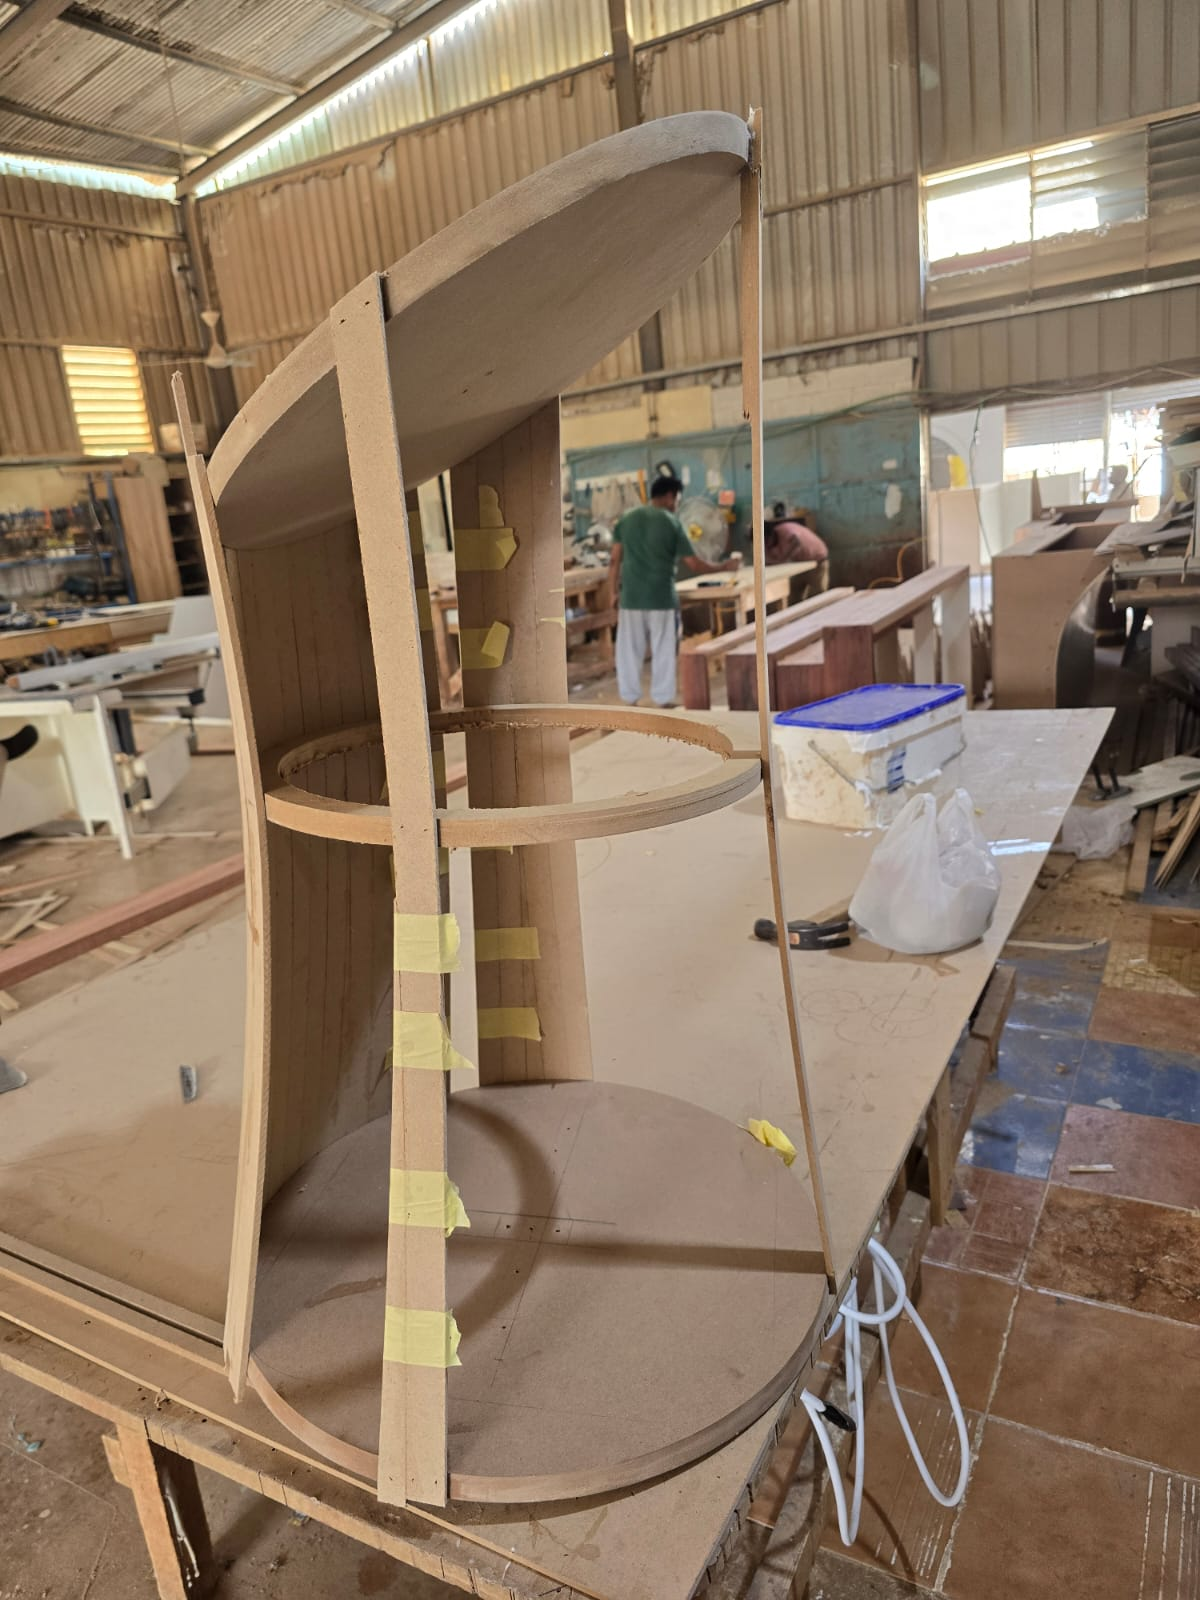
\includegraphics[width=\linewidth,height=5cm,keepaspectratio]{fab_step2.jpeg}
    \caption*{(c) Storage bay and upper frame}
  \end{minipage}
  \caption{Body shell fabrication sequence. MDF circular decks set the profile at each level; thin vertical strips are wetted, bent around the skeleton, and laminated to form the curved surface.}
  \label{fig:fab_sequence}
\end{figure}

\begin{figure}[H]
  \centering
  \begin{minipage}[t]{0.32\linewidth}\centering
    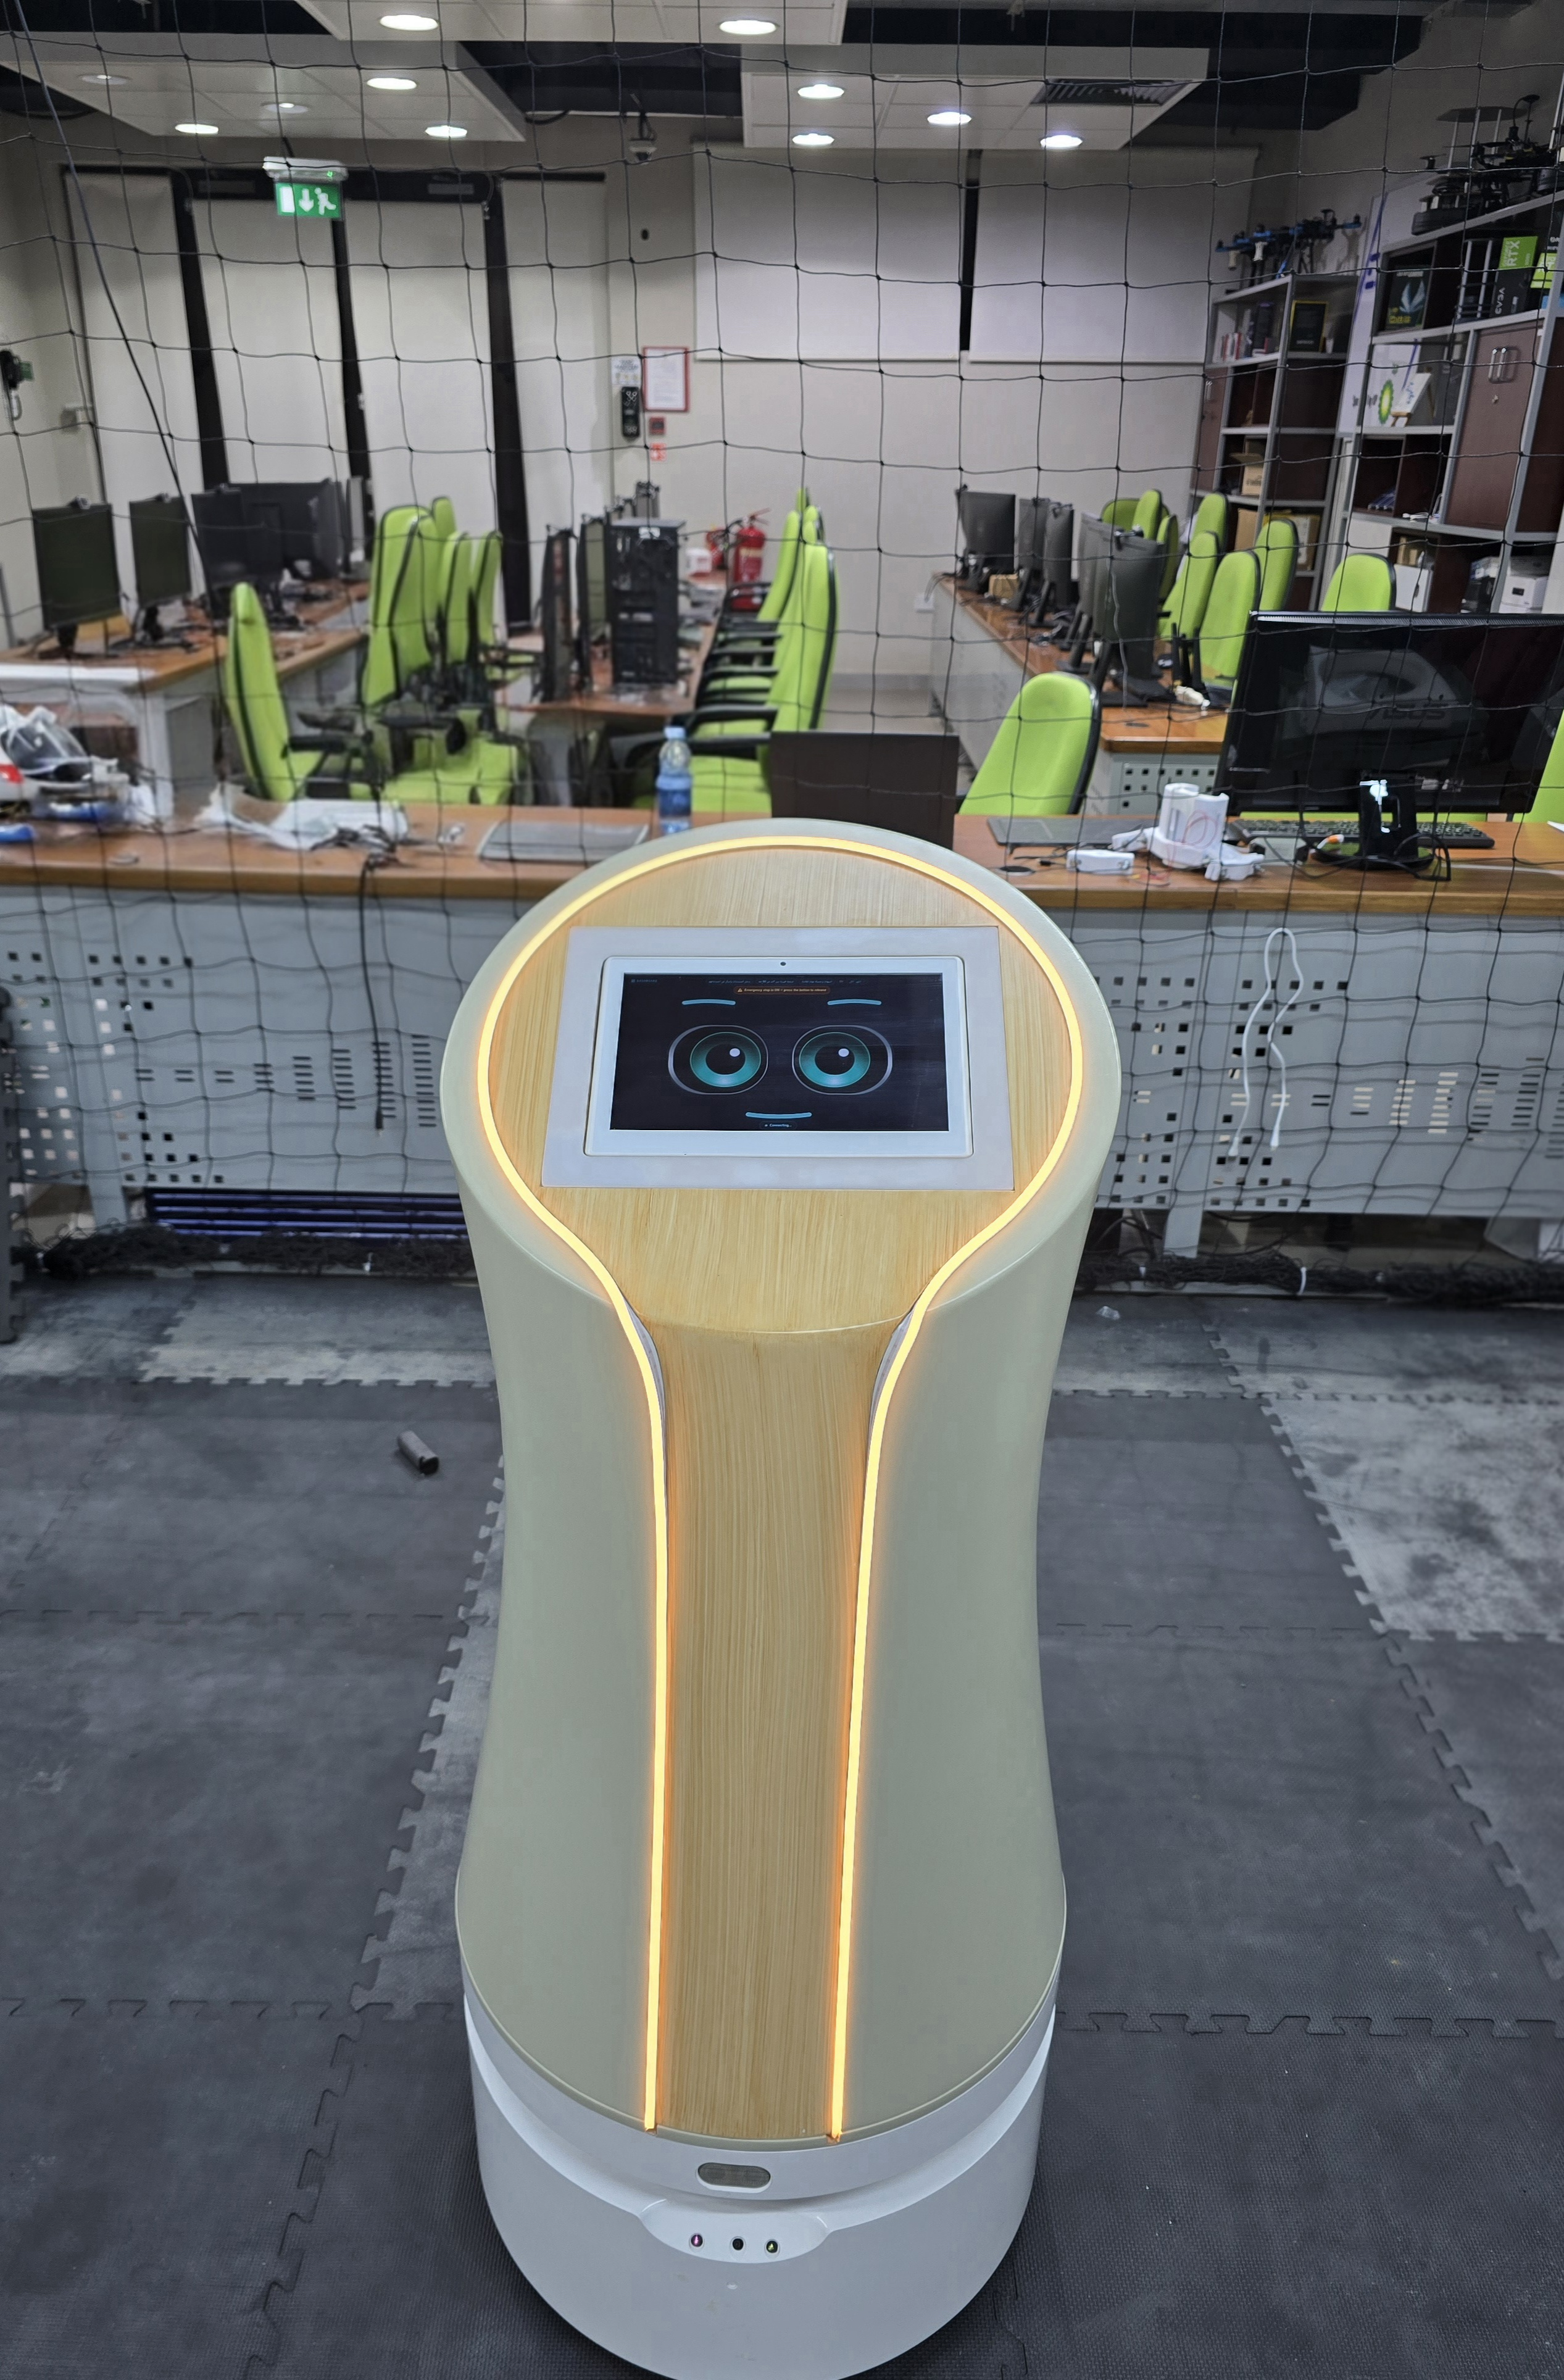
\includegraphics[width=\linewidth,height=6.5cm,keepaspectratio]{robot_front.jpg}
    \caption*{(a) Front view}
  \end{minipage}\hfill
  \begin{minipage}[t]{0.32\linewidth}\centering
    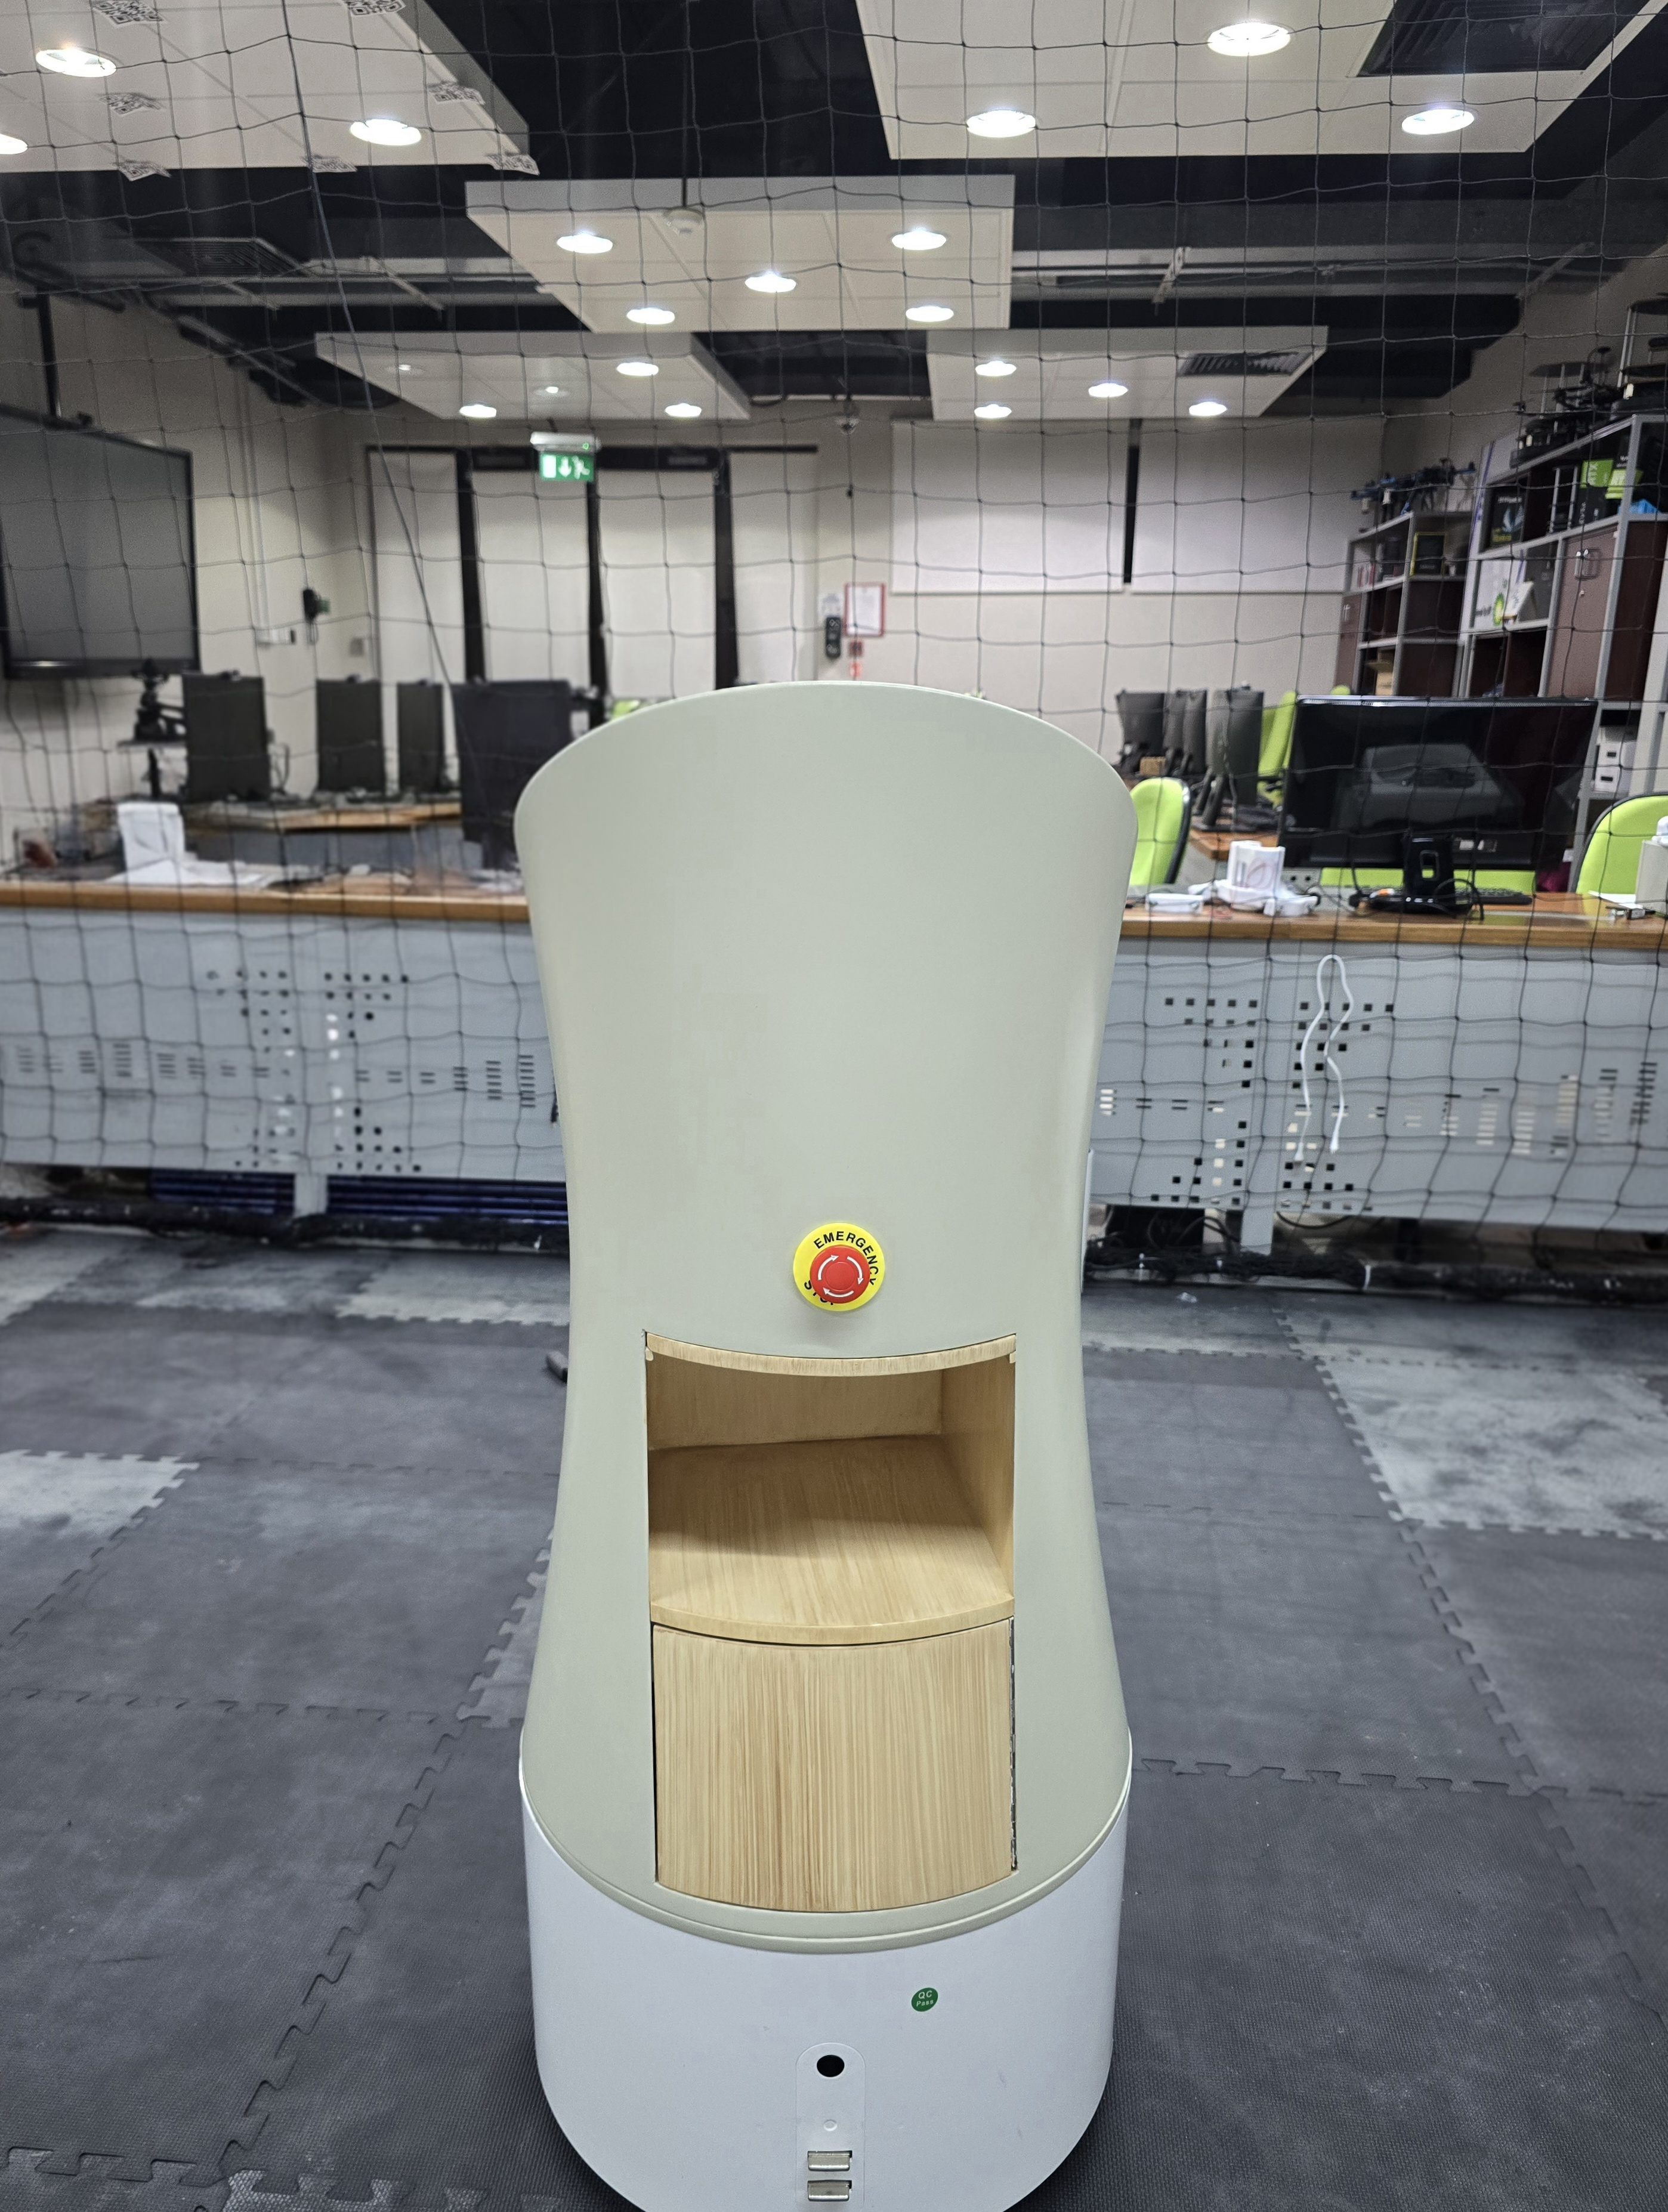
\includegraphics[width=\linewidth,height=6.5cm,keepaspectratio]{robot_rear.jpg}
    \caption*{(b) Rear view}
  \end{minipage}\hfill
  \begin{minipage}[t]{0.32\linewidth}\centering
    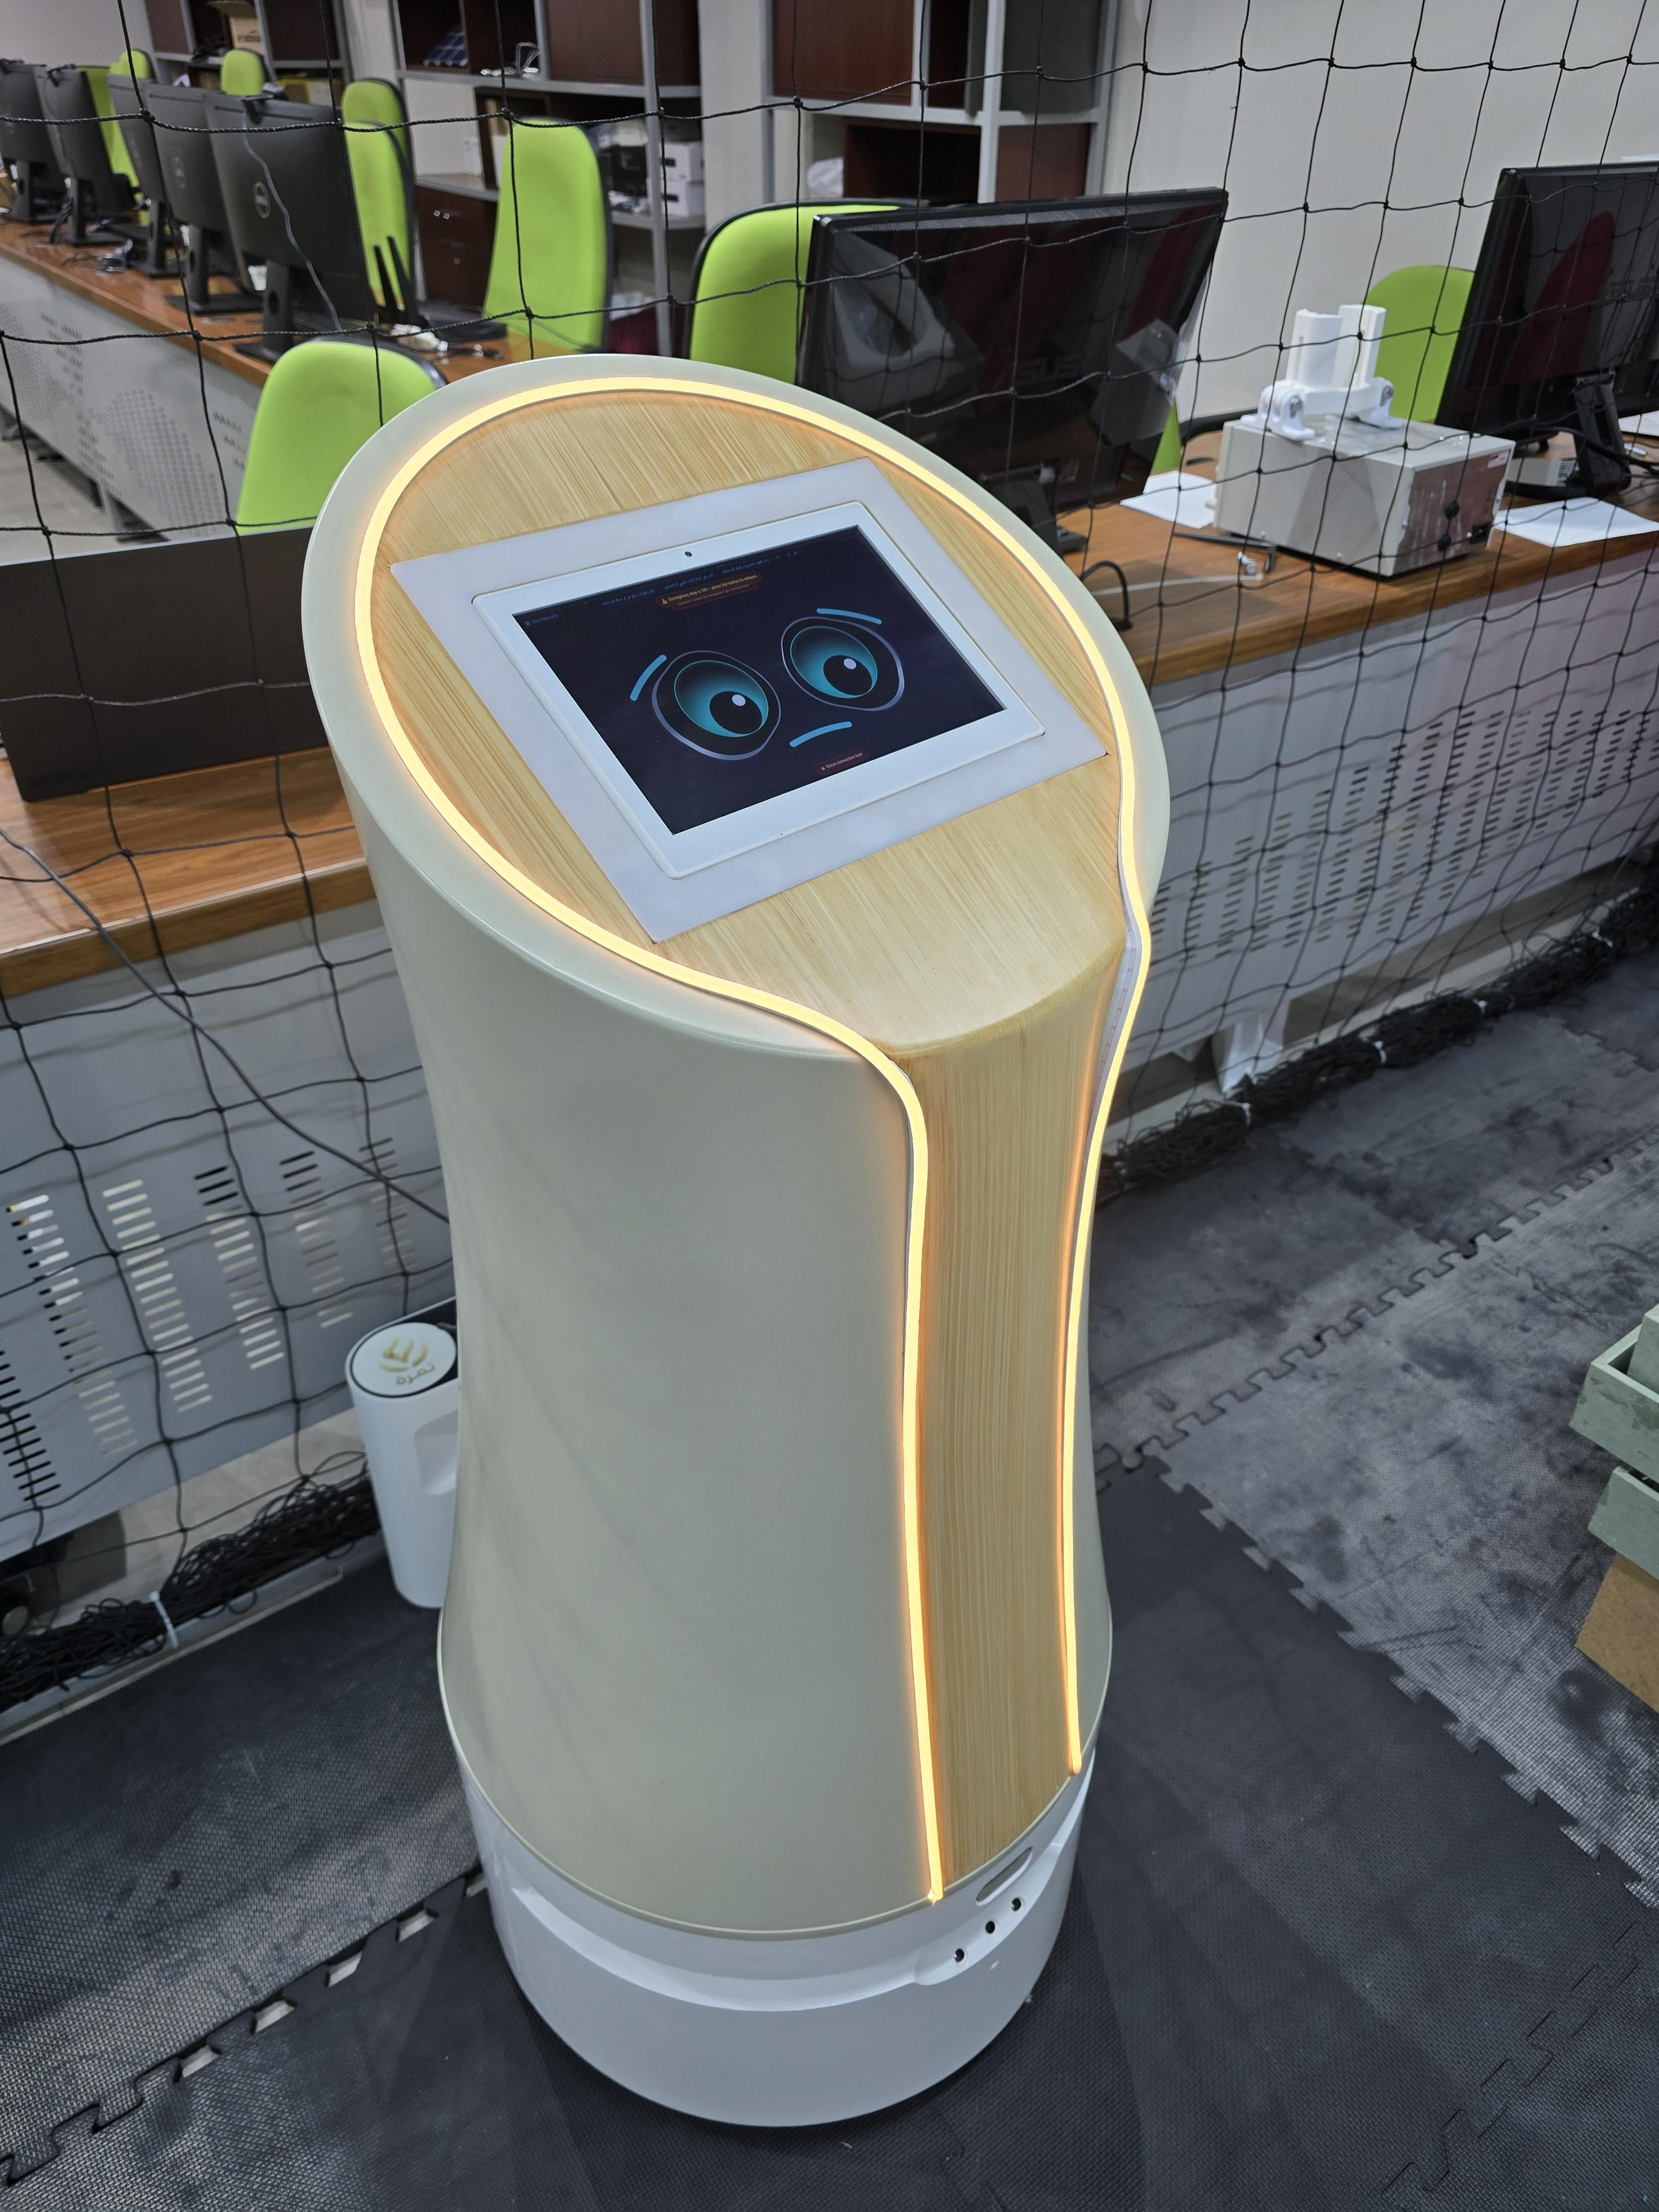
\includegraphics[width=\linewidth,height=6.5cm,keepaspectratio]{robot_top.jpg}
    \caption*{(c) Top view}
  \end{minipage}
  \caption{TAMRA after full integration. Front view (a) shows the oak-veneer panel, ambient LED strip, and the 10-inch display running the animated face. Rear view (b) shows the open storage compartment, oak-veneer drawer, and emergency-stop button. Top view (c) shows the display tilt and overall silhouette.}
  \label{fig:final_robot}
\end{figure}

\subsubsection{Display and Tablet Integration}

The human interface is a 10-inch industrial-grade Android tablet (off-shelf SoC, 2\,GB RAM, 1280$\times$800 IPS touch, Android~11) running in kiosk mode, chosen for always-on operation and extended duty cycle.

\paragraph{Dual-network routing.}
The tablet must simultaneously maintain two network connections: Ethernet to the robot chassis (\texttt{192.168.20.x} subnet) for low-latency ROS WebSocket communication, and Wi-Fi to the campus network for cloud AI APIs and MQTT telemetry. Android's default behaviour routes all traffic over a single interface and drops the other. Eight solutions were evaluated --- dual-channel bonding, an ESP32 MQTT intermediary, a Linux tablet swap, USB Wi-Fi tethering, a 4G/LTE dongle, disabling Wi-Fi, and USB wired tethering --- none reliable or practical. The solution that worked was a boot daemon deployed via ADB (Android Debug Bridge) that sets static routes at startup: traffic to \texttt{192.168.20.x} is forced over \texttt{eth0}; all other traffic uses the \texttt{wlan0} default gateway. The daemon runs at boot and persists across kiosk sessions.

\subsection{Software Implementation}

\subsubsection{Three-Tier Architecture}

The software is structured in three communicating tiers (Figure~\ref{fig:swarch}):

\begin{figure}[H]
  \centering
  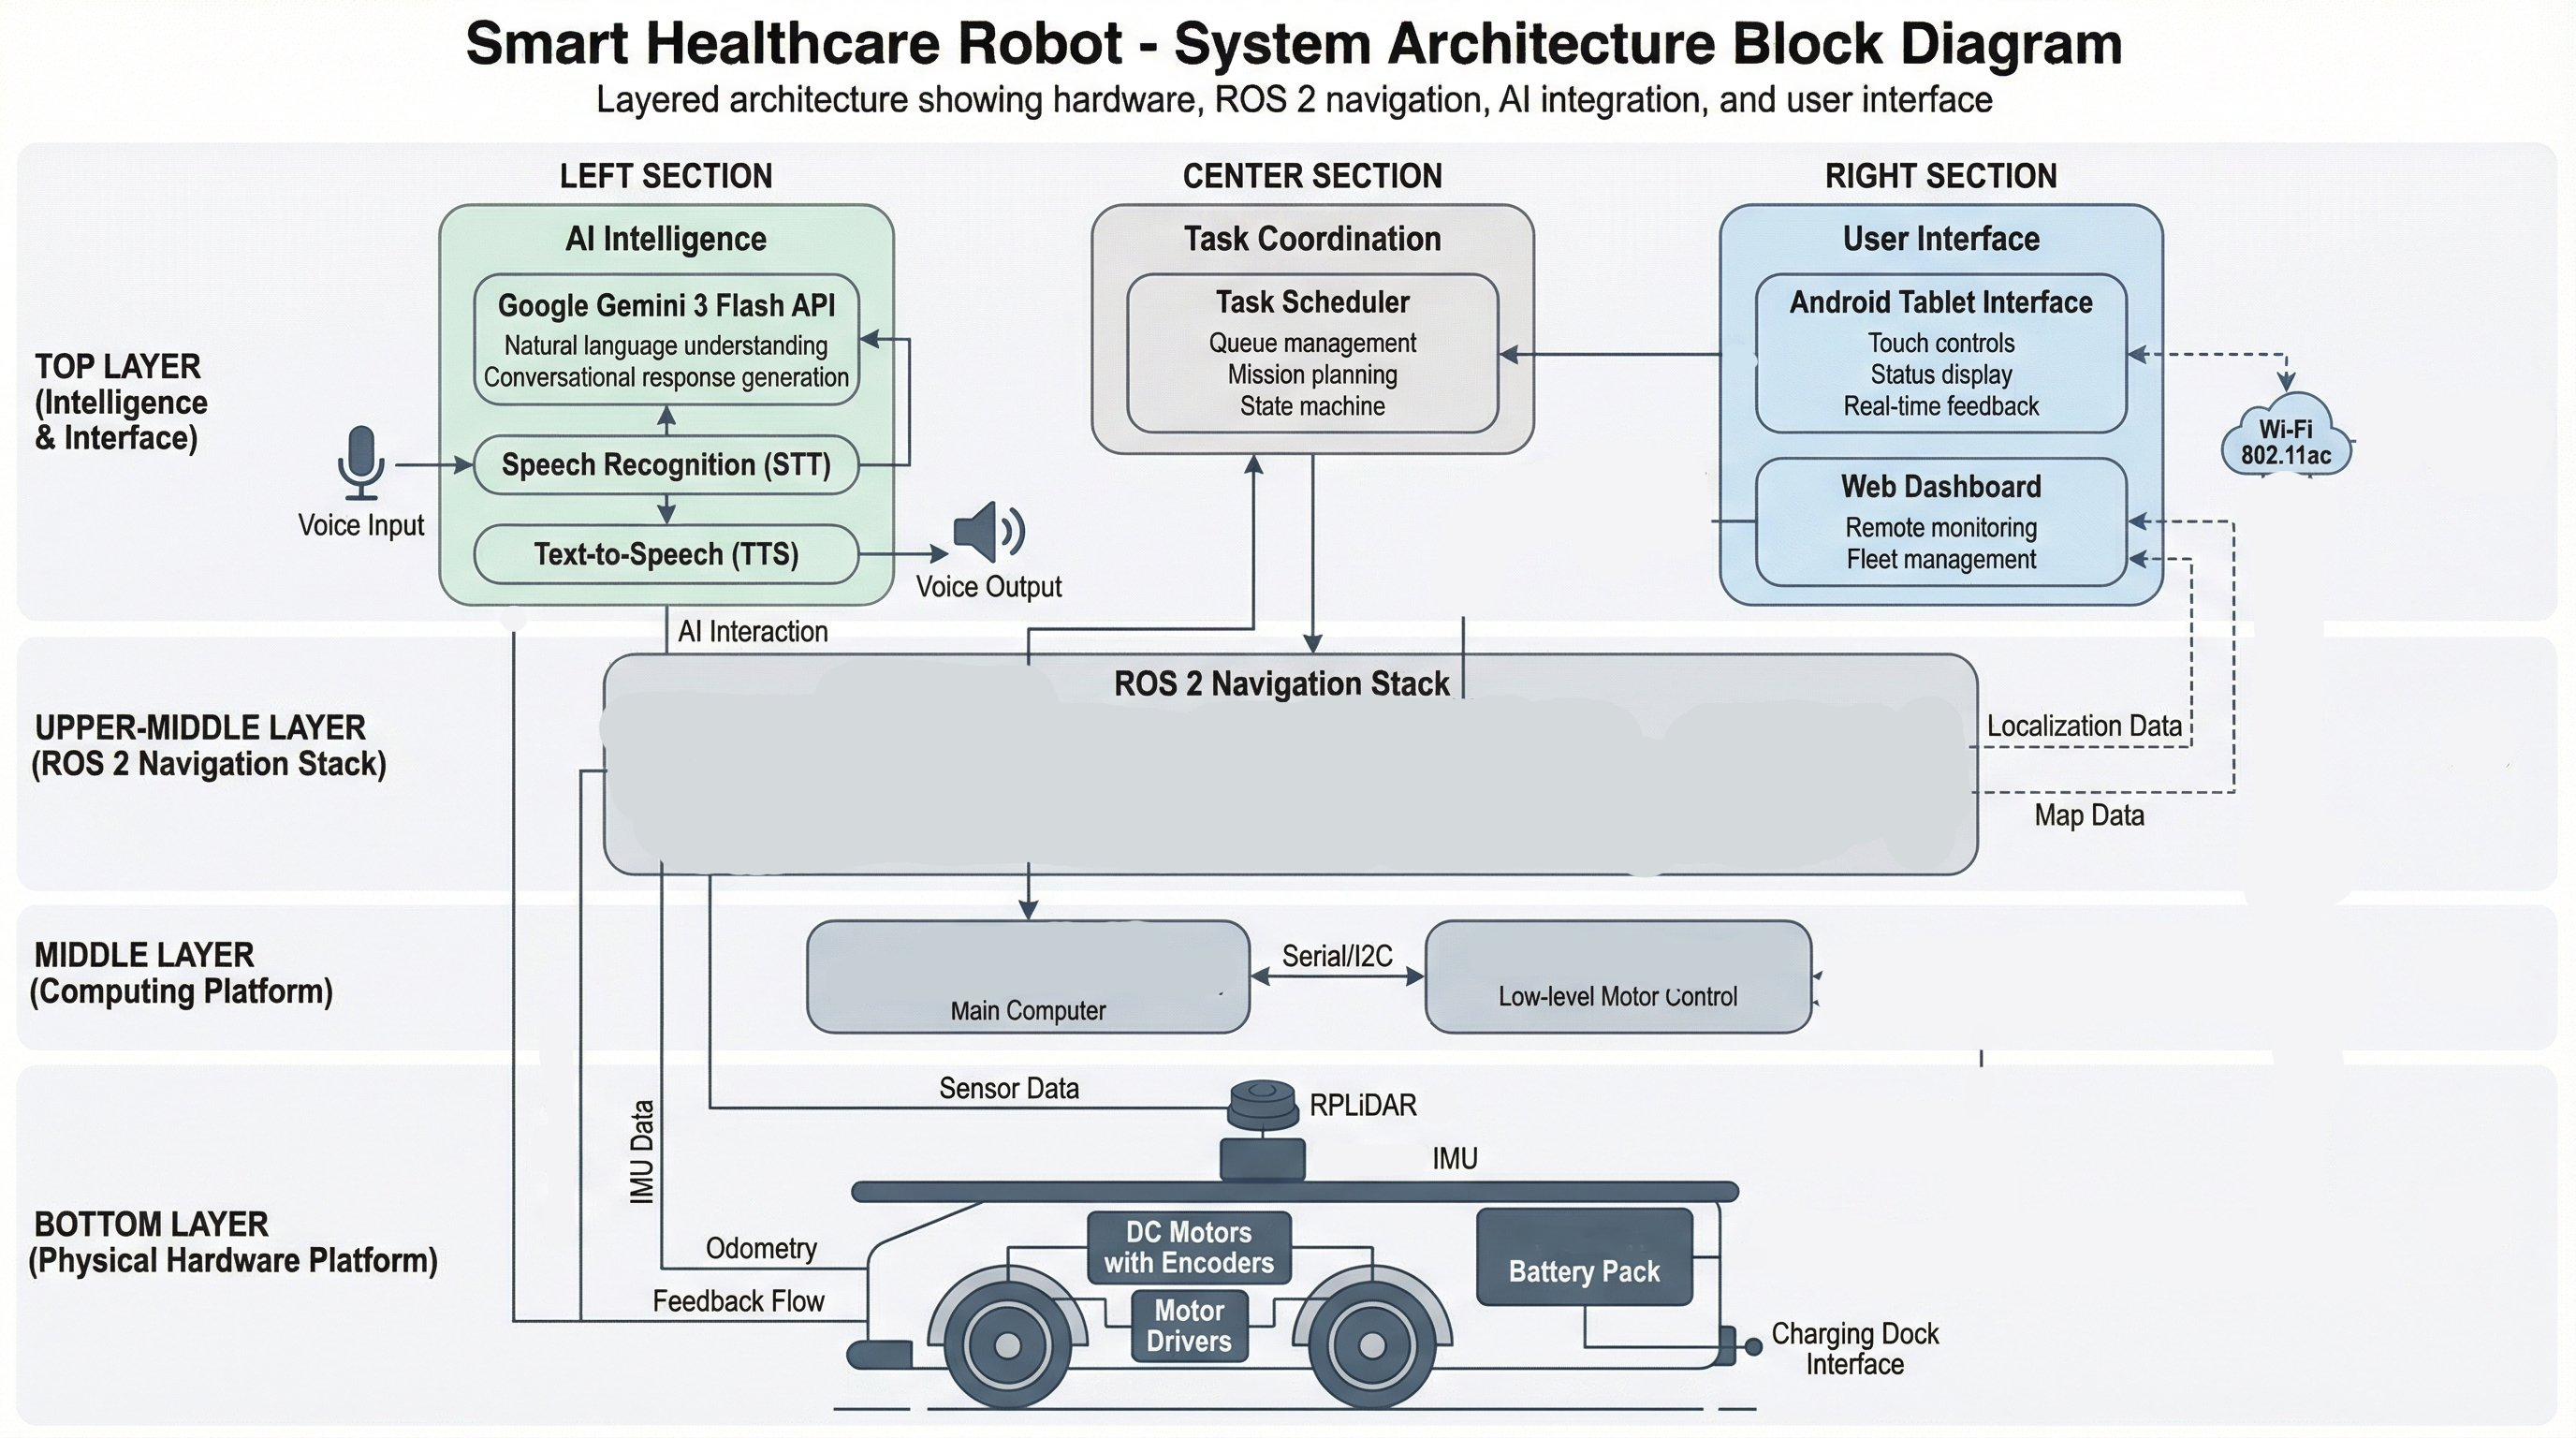
\includegraphics[width=0.92\textwidth]{system_block.png}
  \caption{Three-tier software architecture. The Robot Layer (iMRP500 SoC) runs ROS navigation and exposes sensor data over WebSocket. The Bridge Layer (tablet) hosts the mission engine, voice pipeline, and MQTT bridge. The Cloud Layer provides LLM orchestration, voice synthesis, and remote telemetry.}
  \label{fig:swarch}
\end{figure}

\begin{itemize}
  \item \textbf{Robot Layer}: The iMRP500 onboard SoC runs the ROS navigation stack, sensor drivers, and costmap pipeline. It exposes the rosbridge WebSocket on port~9090 and MJPEG video on port~9099.
  \item \textbf{Bridge Layer}: The tablet application --- a single self-contained HTML file --- connects to the robot over Ethernet WebSocket and to the cloud over Wi-Fi. It hosts the mission engine, task queue, cron scheduler, MQTT bridge, and the animated face. A single file requires no installation and can be updated by replacing it over ADB.
  \item \textbf{Cloud Layer}: Google Gemini~3 Flash provides LLM orchestration; a conversational-AI service provides speech recognition and synthesis; HiveMQ Cloud provides TLS-encrypted MQTT brokering for remote telemetry and control.
\end{itemize}

\subsubsection{Semantic Task Orchestrator}

The orchestrator is the core software contribution of the project. It implements long-horizon task orchestration: a user speaks or types a natural-language command in English or Arabic --- for example, ``take this to the pharmacy, then go check on room 5 and come back'' --- and the orchestrator converts it into a structured, executable sequence of robot actions spanning multiple locations, multiple steps, and multiple minutes of autonomous operation, with no further human input.

The orchestrator invokes Gemini~3 Flash with a prompt that includes live robot context --- battery level, current position, known waypoints, and active task queue --- as dynamic variables. The model returns a typed mission plan:
\begin{equation}
  s_i \in \{\,\texttt{navigate}(w),\;\texttt{speak}(m),\;\texttt{display}(d),\;\texttt{photo},\;\texttt{wait}(t)\,\}
\end{equation}
where $w$ is a named waypoint, $m$ a spoken message, $d$ display content, and $t$ a wait duration. The plan is returned as a server-sent event (SSE) stream, and the mission engine begins executing the first step before the full plan is generated. This streaming execution means the robot starts moving while the model is still producing later steps --- the primary mechanism for keeping voice-to-action latency below 3\,s.

\subsubsection{Voice Pipeline}

Three voice configurations were prototyped:
\begin{enumerate}
  \item An OpenAI live model: functional, but voice quality and tool-call latency felt unnatural in practice.
  \item A standalone synthesis service: more natural voice, but overall round-trip latency was perceived as slow when combined with ROS command dispatch.
  \item \textbf{Gemini~3.1 Live (current)}: real-time bidirectional audio with native tool-calling, eliminating the layered latency of the previous configurations. Tool calls (\texttt{robot\_control}, \texttt{plan\_and\_execute}, \texttt{cancel\_mission}) route directly to client-side handlers on the robot bridge.
\end{enumerate}

\subsubsection{Task Queue and Mission Engine}

The mission engine maintains a priority queue with five states:
\[
\textsc{pending} \;\to\; \textsc{running} \;\to\; \{\,\textsc{completed},\;\textsc{failed},\;\textsc{cancelled}\,\}
\]
A 1\,Hz tick dispatches navigation goals via the \texttt{/poi} ROS service. Four mission types are supported: \textbf{GO\_TO} (single-waypoint), \textbf{DELIVERY} (multi-stop sequence of up to five waypoints with confirmation at each stop), \textbf{PATROL} (looping route through points of interest), and \textbf{AUTO\_CHARGE} (battery-triggered return to dock, default threshold 20\%). A built-in cron scheduler accepts standard five-field POSIX expressions for recurring autonomous missions.

\subsubsection{MQTT Bridge and Remote Dashboard}

Robot state is published at 1\,Hz over HiveMQ Cloud (WSS, TLS): pose, battery percentage, task queue, and navigation status. Telemetry uses MQTT QoS~1 (at-least-once) to guarantee state updates under transient packet loss; control commands use QoS~2 (exactly-once) to prevent duplicate navigation goals. Large payloads (occupancy grid maps) are chunked into 64\,KB segments. The React-based remote dashboard renders a live occupancy grid map with robot pose overlay, task-creation interfaces, task-queue monitoring, cron management, and a live MJPEG camera view for telepresence. Communicating exclusively over MQTT, it operates from any internet-connected device without VPN or special routing.

\subsubsection{Electrical Integration}

The added hardware (tablet, display, LED strip, kill switch) draws power from the iMRP500 chassis through a single regulated bus. The chassis exposes three external interfaces: a 24\,V power terminal, a hardware kill-switch terminal pair, and an Ethernet port. A 3\,A fuse protects the downstream rail; a DC--DC step-down converter regulates 24\,V to 12\,V for the tablet and the LED strip. The physical kill switch is wired normally-open (NO) so that pressing it breaks the chassis safety loop and halts the drive motors per ISO~13850. Figure~\ref{fig:wiring} shows the wiring topology.

\begin{figure}[H]
\centering
\fcolorbox{black}{black}{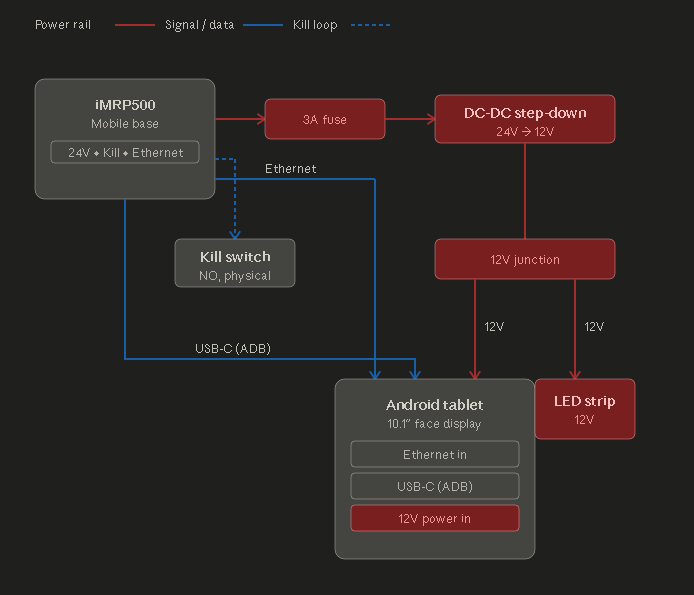
\includegraphics[width=0.65\linewidth]{wiring_diagram.png}}
\caption{TAMRA electrical integration. The kill switch is wired NO so activation opens the chassis safety loop per ISO~13850. The 24\,V rail passes through a 3\,A fuse and a DC--DC step-down converter to supply 12\,V to the tablet and LED strip. Three connections enter the tablet: 12\,V power, Ethernet from the chassis, and a persistent ADB USB link used by the dual-network boot daemon and for over-the-air HTML updates.}
\label{fig:wiring}
\end{figure}

\subsection{System Integration and Testing}

\subsubsection{Unit Tests}

Each subsystem was validated independently before integration:
\begin{itemize}
  \item \textbf{Navigation}: SLAM mapping completed; waypoint navigation confirmed $\pm$5\,cm accuracy; all four costmap layers verified against static and moving test obstacles.
  \item \textbf{Sensor pipeline}: All topics confirmed over the WebSocket bridge; the self-diagnosis service returned healthy status for LiDAR, network, encoders, battery, IR, ultrasonic, gyro, and depth camera.
  \item \textbf{Orchestrator}: Fifteen natural-language commands of increasing complexity (single waypoint, multi-stop delivery, conditional return) were submitted in isolation; all fifteen produced valid, executable plans, with the first SSE step delivered within 1.2\,s on average.
  \item \textbf{Voice pipeline}: Tested for intelligibility, tool routing, and mid-speech interruption handling; all three tool calls routed correctly.
  \item \textbf{Body shell}: Footprint within 500\,mm confirmed; total height 900\,mm; added mass below 12\,kg; display tilt verified at 40$^{\circ}$; storage compartment functional; no sharp edges.
\end{itemize}

\subsubsection{Integration and Acceptance Testing}

The acceptance test validated all six customer requirements in a continuous sequence. A delivery mission was issued by voice: the robot navigated to a waypoint, announced its arrival verbally, waited for confirmation, then returned to the docking station and initiated autonomous charging. Remote control was exercised simultaneously from the MQTT dashboard on a separate device. A voice-interruption test confirmed that an in-flight patrol mission could be cancelled and replaced with a new navigation goal within 2\,s of the voice command. All engineering requirements were met within the applicable constraints, including the 300\,OMR body-shell budget, the 500\,mm chassis footprint, the 12\,kg added-mass limit, and the ISO~13482 and ISO~13850 safety standards.

\subsection{Results}
\label{sec:results}

\subsubsection{Voice-to-Action Latency}

End-to-end latency from voice-command completion to first robot motion was measured across 20 trials ($N=20$). Figure~\ref{fig:latency_bar} shows the per-component breakdown.

\begin{figure}[H]
\centering
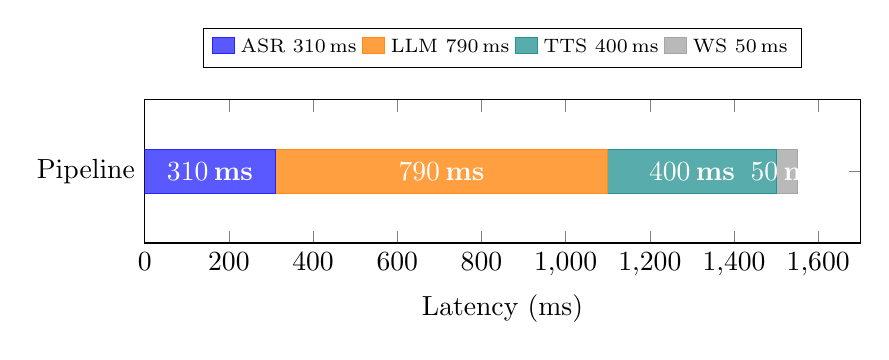
\begin{tikzpicture}
\begin{axis}[
    xbar stacked, width=0.88\linewidth, height=3.4cm,
    xlabel={Latency (ms)}, ytick={1}, yticklabels={Pipeline},
    xmin=0, xmax=1700, ymin=0.3, ymax=1.7, bar width=16pt,
    legend style={at={(0.5,1.22)},anchor=south,legend columns=4,font=\scriptsize},
    enlarge y limits=0.5,
    nodes near coords={\pgfmathprintnumber\pgfplotspointmeta\,ms},
    every node near coord/.append style={font=\tiny,text=white,font=\bfseries},
]
\addplot[fill=blue!65,draw=blue!85]     coordinates {(310,1)};
\addplot[fill=orange!75,draw=orange!90] coordinates {(790,1)};
\addplot[fill=teal!65,draw=teal!85]     coordinates {(400,1)};
\addplot[fill=gray!55,draw=gray!70]     coordinates {( 50,1)};
\legend{ASR 310\,ms, LLM 790\,ms, TTS 400\,ms, WS 50\,ms}
\end{axis}
\end{tikzpicture}
\caption{Voice-to-action latency breakdown ($N=20$, mean total 1{,}550\,ms, $\sigma=310$\,ms). LLM tool-call resolution dominates at 51\%. All 20 trials completed below the 3\,s engineering requirement (max observed 2.41\,s). Streaming SSE execution further reduces perceived latency by dispatching the first navigation command before the complete plan is generated.}
\label{fig:latency_bar}
\end{figure}

\subsubsection{MQTT Telemetry Latency}

Round-trip latency between the robot bridge and HiveMQ Cloud was measured over 30 timestamped message pairs ($N=30$). Figure~\ref{fig:mqtt_hist} shows the distribution.

\begin{figure}[H]
\centering
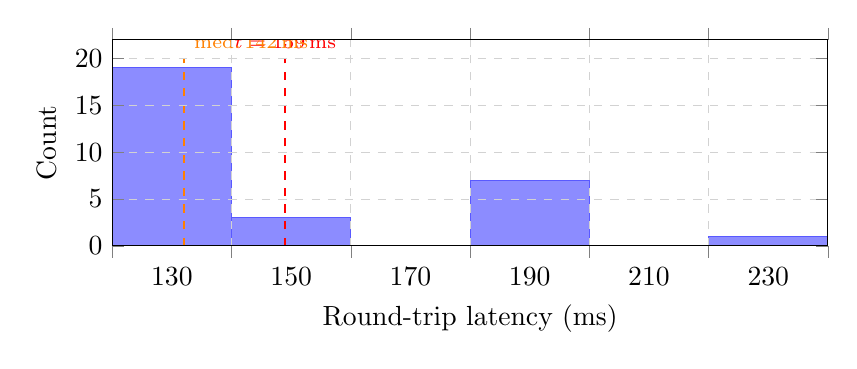
\begin{tikzpicture}
\begin{axis}[
    ybar interval, width=0.88\linewidth, height=4.2cm,
    xlabel={Round-trip latency (ms)}, ylabel={Count},
    xmin=130, xmax=250, ymin=0, ymax=22,
    xtick={130,150,170,190,210,230,250},
    ymajorgrids=true, grid style={dashed,gray!35}, area style,
]
\addplot[fill=blue!45,draw=blue!65] coordinates {
    (130,19)(150,3)(170,0)(190,7)(210,0)(230,1)(250,0)
};
\draw[dashed,red,thick] (axis cs:159,0)--(axis cs:159,20)
    node[above,font=\scriptsize,red]{$\bar{t}=159$\,ms};
\draw[dashed,orange,thick] (axis cs:142,0)--(axis cs:142,20)
    node[above right,font=\scriptsize,orange]{med.\,142\,ms};
\end{axis}
\end{tikzpicture}
\caption{MQTT round-trip latency distribution ($N=30$). Mean 159\,ms, median 142\,ms, 95th percentile 207\,ms, max 243\,ms. All 30 messages delivered below 250\,ms. The bimodal distribution reflects occasional deep-packet-inspection buffering on the campus Wi-Fi; direct robot control uses the local Ethernet path and is unaffected. Telepresence video latency (MJPEG stream) was separately measured at 130\,ms under the same conditions.}
\label{fig:mqtt_hist}
\end{figure}

\subsubsection{Navigation and Orchestrator}

Waypoint navigation accuracy of $\pm$5\,cm was confirmed through repeated trials across three defined waypoints. The four-layer costmap successfully avoided all static and dynamic test obstacles. All fifteen orchestrator test commands produced valid, executable mission plans with no hallucinated waypoints or malformed step types.

\subsection{Budget Summary}

\begin{table}[H]
\centering
\small
\caption{Hardware procurement costs.}
\label{tab:budget}
\setlength{\tabcolsep}{6pt}
\begin{tabular}{@{} >{\raggedright\arraybackslash}p{6.0cm} r @{}}
\toprule
\textbf{Item} & \textbf{OMR} \\
\midrule
iMRP500 chassis (incl.\ shipping)         & 850 \\
10-inch 1080p industrial touch display    & 77 \\
Body shell (MDF, veneer, acrylic, paint)  & 300 \\
Cables, fasteners, connectors             & 73 \\
\midrule
\textbf{Total}                            & \textbf{1{,}300} \\
\bottomrule
\end{tabular}
\end{table}

\noindent At approximately USD~3{,}200, TAMRA delivers autonomous navigation, conversational AI, item delivery, and remote telepresence --- a 73\% cost reduction against the nearest commercial platform with comparable capability~\cite{pudubot2,m2medical}.

\subsection{Standards Compliance}

\begin{itemize}
  \item \textbf{ISO~13482:2014}: Navigation speed (0.8\,m/s) and inflation radius (0.8\,m) satisfy the velocity and proximity limits for robots in human-shared spaces.
  \item \textbf{ISO~13850}: Hardware E-stop relay tested; the robot halts within one control cycle on activation. A soft-stop service provides a software-level equivalent.
  \item \textbf{ITU-T~H.264}: Camera streams use standard compressed formats compatible with web browsers.
  \item \textbf{IEEE~802.11}: MQTT and cloud AI APIs operate over standard Wi-Fi with no infrastructure modifications.
\end{itemize}

\subsection{Section Summary}

This section documented the full implementation of TAMRA. The iMRP500 was selected after a six-platform comparison and reverse-engineered to expose its full sensor suite over a documented WebSocket API. The body shell was designed through a three-stage workflow --- concept rendering, AI-assisted 3D mesh synthesis, and parametric Fusion~360 refinement --- and fabricated locally within budget and mass constraints. The three-tier software stack was developed in parallel with hardware procurement. Measured results confirm voice-to-action latency of $1{,}550 \pm 310$\,ms (all 20 trials below 3\,s), MQTT round-trip of $159 \pm 30$\,ms, navigation accuracy of $\pm$5\,cm, and 100\% plan-generation success across 15 orchestrator test commands.

% ============================================================
% 6. CONCLUSIONS AND FUTURE WORK  (trimmed)
% ============================================================
\section{Conclusions and Future Work}
\label{sec:conclusion}

\subsection{Project Summary}

This project produced TAMRA (Task-Agnostic Modular Robotic Apparatus), an autonomous mobile robot that integrates LiDAR-based navigation, LLM-driven semantic task orchestration, real-time voice interaction, item delivery, and remote telepresence on a single platform at a total hardware cost of approximately USD~3{,}200. The work spanned two semesters: the first built the design foundation through literature review, requirements formalisation, and AHP-based architecture selection; the second realised the system, navigating two significant decisions --- a platform transition forced by a supplier bankruptcy and the structural limits of educational bases, and a scope refinement from a strictly medical device to a general-purpose service robot, validated in a healthcare corridor but designed to generalise. That reframing was the difference between a system deployable within the project timeline and one that was not.

\paragraph{Technical contributions.}
\begin{enumerate}
  \item \textbf{Hybrid hardware platform}: an industrial chassis combined with a custom-fabricated ergonomic body shell built within a 300\,OMR budget. The design workflow --- generative rendering to 3D mesh synthesis to parametric Fusion~360 refinement --- is a reproducible methodology for human-facing robot aesthetics, in which the AI-generated mesh served as a starting reference that required substantial engineering correction.
  \item \textbf{Semantic task orchestrator}: a streaming LLM pipeline that converts free-form English or Arabic voice commands into typed, multi-step mission plans executed in real time by an on-device mission engine, with measured voice-to-action latency of $1{,}550 \pm 310$\,ms ($N=20$, all trials below 3\,s).
  \item \textbf{Layered software architecture}: a three-tier stack (ROS~2 navigation, tablet bridge application, cloud AI and MQTT telemetry) that separates concerns cleanly and allows the full system to be updated by replacing a single HTML file over ADB.
\end{enumerate}

\subsection{Areas for Improvement}
\begin{itemize}
  \item \textbf{High-traffic navigation}: the global planner replans inefficiently when many moving obstacles appear simultaneously; a more adaptive local planner or an upgraded dynamic-obstacle layer would improve fluency~\cite{chen2022}.
  \item \textbf{Voice recognition in noise}: ASR accuracy degrades in noisy reception areas; a directional microphone array or server-side noise suppression would address this.
  \item \textbf{Autonomous docking}: localisation drift over a long shift can cause missed dock contact; a short-range UWB or IR beacon for fine-approach correction would reach the 95\% docking target.
  \item \textbf{Arabic coverage}: the orchestrator and voice pipeline support Arabic, but systematic accuracy evaluation with native speakers remains to be completed.
\end{itemize}

\subsection{Future Work}
Planned extensions include licence-free 433\,MHz hardware call buttons for summoning the robot without a phone or network; WhatsApp Business Cloud API integration for summoning, delivery requests, and status checks through an application already ubiquitous in the region; multi-robot fleet coordination using the existing MQTT topic-namespace architecture and ROS~2's DDS layer; Hospital Information System integration via HL7/FHIR so the orchestrator can read room assignments and schedules dynamically~\cite{jmir2024}; an optional UV-C disinfection module with occupancy-gated safety interlocks~\cite{sciencedirect2021}; and a longitudinal field study in a hospital, hotel, or campus building to measure navigation reliability, staff workflow impact, and maintenance burden before broader rollout.

% ============================================================
% REFERENCES
% ============================================================
\newpage
\bibliographystyle{unsrt}
\bibliography{references/references}

\end{document}
